Figure \ref{fig:img2_src} shows Image 2, which is the original image filled with black and white pixels. This kind of noise is known as salt--and--pepper noise, and from the image's histogram (figure \ref{fig:img2_hist}) can the amount of salt--and--pepper noise be seen; salt noise on the right and pepper noise on the left. 
\begin{figure}[H]
    \centering
    \begin{subfigure}[b]{0.25\textwidth}
        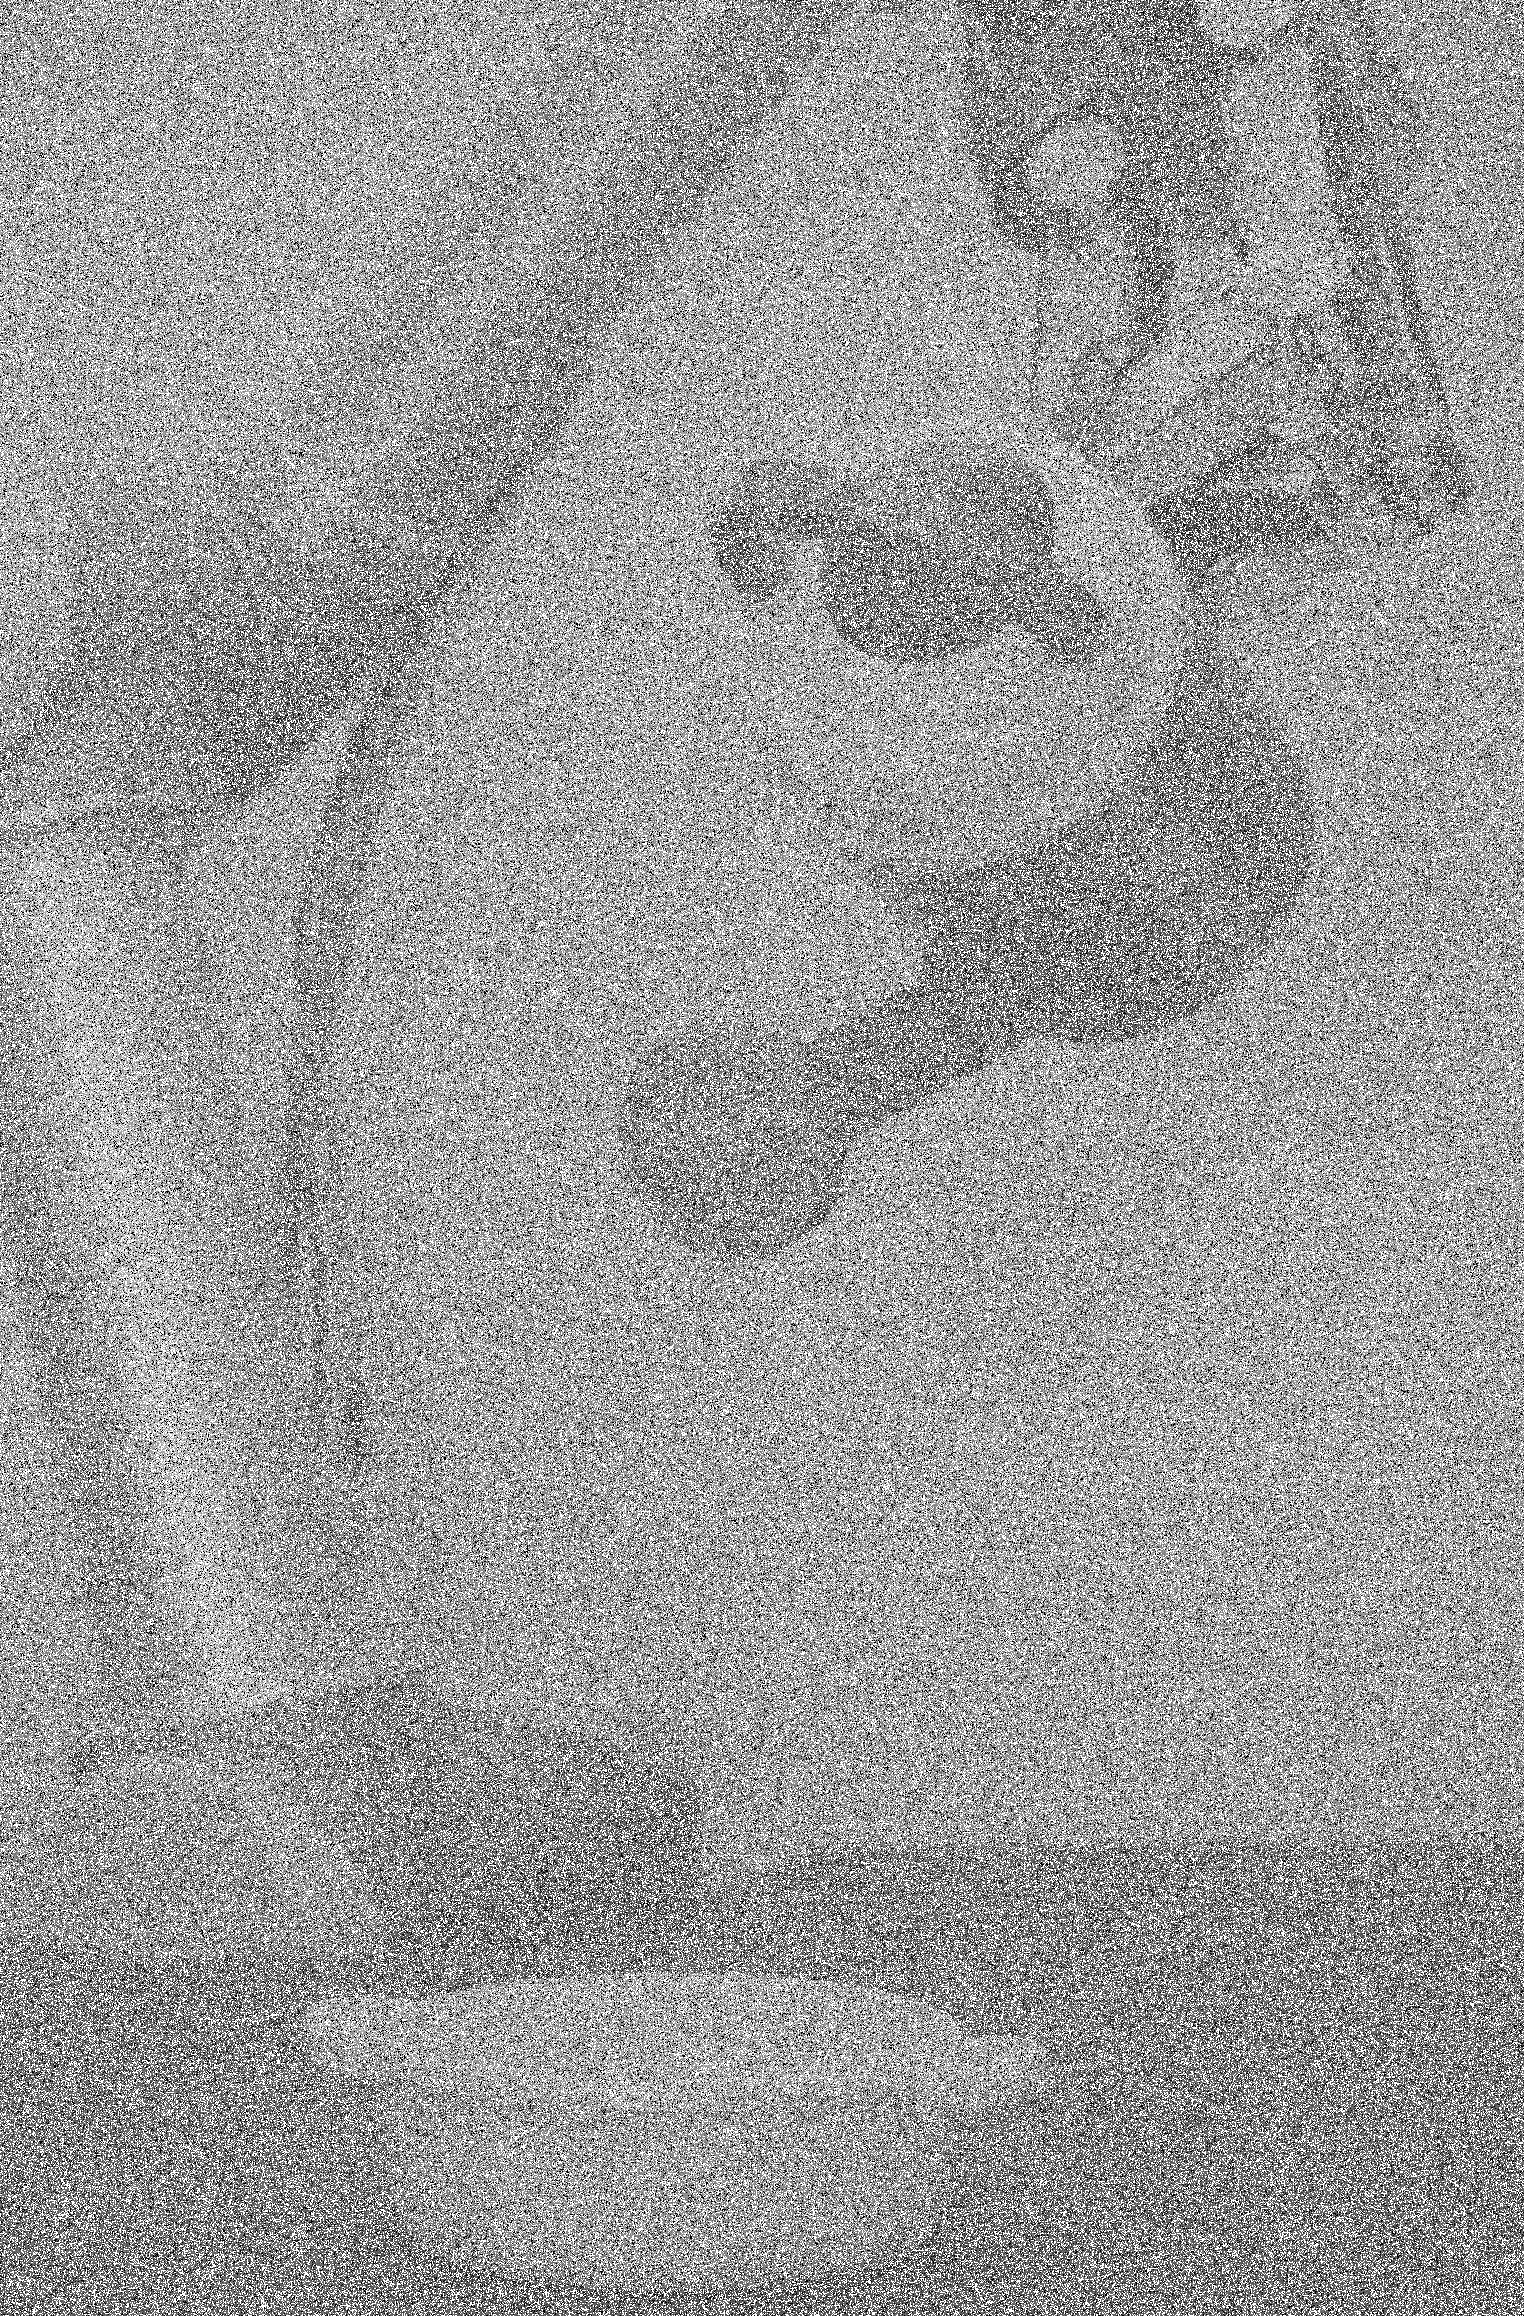
\includegraphics[width=\textwidth]{img2/src.png}
        \caption{The original image}
        \label{fig:img2_src}
    \end{subfigure}
    \begin{subfigure}[b]{0.485\textwidth}
        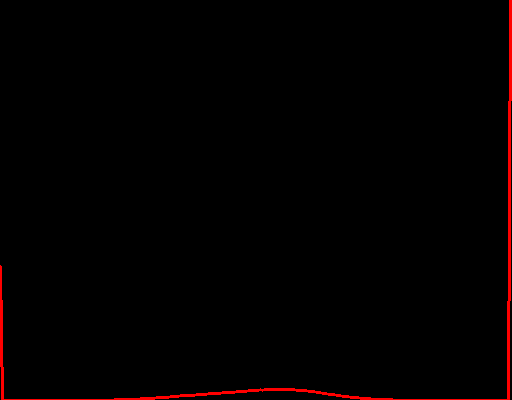
\includegraphics[width=\textwidth]{img2/hist_org_img2.png}
        \caption{Histogram of the original image}
        \label{fig:img2_hist}
    \end{subfigure}
    \caption{Analysis of image 2}\label{fig:img2}
\end{figure}

In order to better see the effect of the salt--and--pepper noise, a uniform surface (figure \ref{fig:rect_org_img2}) is analysed, in this case the red square marked on figure \ref{fig:src_square}. The histogram of the uniform surface is shown on figure \ref{fig:hist_rect_org_img2}, and here is the salt--and--pepper noise also clear to see. 
\begin{figure}[H]
    \centering
    \begin{subfigure}[b]{0.22\textwidth}
        \includegraphics[width=\textwidth]{img2/src_square.png}
        \caption{The original image}
        \label{fig:src_square}
    \end{subfigure}
        \begin{subfigure}[b]{0.335\textwidth}
        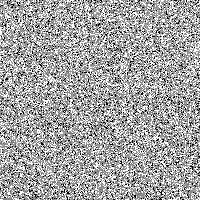
\includegraphics[width=\textwidth]{img2/rect_org_img2.png}
        \caption{The uniform surface}
        \label{fig:rect_org_img2}
    \end{subfigure}
    \begin{subfigure}[b]{0.43\textwidth}
        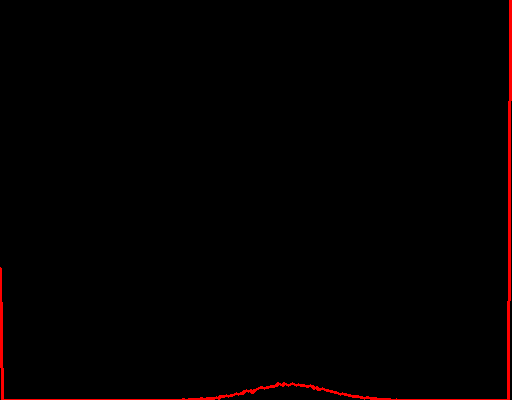
\includegraphics[width=\textwidth]{img2/hist_rect_org_img2.png}
        \caption{Histogram of the uniform surface}
        \label{fig:hist_rect_org_img2}
    \end{subfigure}
    \caption{Analysis of an uniform surface of image 2}\label{fig:img2_rect}
\end{figure}

Approximately are there three times more salt noise compared to the pepper noise. The values in the middle of the histogram is what is left of the original image, and in order to restore as much as possible, and median filter is applied on the image. The median filter is chosen because it is very effective against salt-and-pepper noise in the images, and the OpenCV function
\begin{center}
\lstinline|void medianBlur(InputArray src, OutputArray dst, int ksize)|\footnote{\url{http://docs.opencv.org/2.4/modules/imgproc/doc/filtering.html\#void medianBlur(InputArray src, OutputArray dst, int ksize)}}
\end{center}
is used for applying the filter to the image. Basically the image blurred by using the median filter, and depending on the size of \lstinline|ksize|, the more blurred will the image become.\\[0.2cm]
The \lstinline|ksize| is the size of the kernel filter applied to each pixel in the image, and therefore must the value of \lstinline|ksize| be odd and greater than 1, so in order to test if the noise is removed, a kernel of \lstinline|3| is applied on the image 2 and checked if all the noise is removed. If not all the noise is removed, the kernel size is increased with two, and checked again, and so on. In order to better see the reduction of the noise by using the the \lstinline|medianBlur|, the same method used in figure \ref{fig:img2_rect} are applied after using each kernel filter, becuase it is easier to see the reduction of the noise on the uniform surface. From the uniform surfaces histograms can it be seen that the more compact the peak get, the lesser noise are there in the picture and the more uniform gets the color of the surface.\\[0.2cm]
Figure \ref{fig:img2_kernel3}, \ref{fig:img2_kernel5}, \ref{fig:img2_kernel7} and \ref{fig:img2_kernel9} shows the process of finding the right \lstinline|ksize|, but all four kernel sizes still does not remove all the noise, especially the salt noise. All the salt--and--pepper noise is removed with a \lstinline|ksize=11|, but the disadvantage of this approach is that the details in the image are reduced. For restoring as much as possible of the these details, a histogram equalization is applied on the noise reduced image. Histogram equalization restores the details by improves the contrast in the image by stretching out the intensity range of the image. On the left and right side of image \ref{fig:img2_kernel11}'s histogram are there underpopulated intensities, which is why an histogram equalization is an optimal choice. The result is shown on figure \ref{fig:img2_histEq}.

\begin{figure}[H]
    \centering
    \begin{subfigure}[b]{0.24\textwidth}
        \includegraphics[width=\textwidth]{img2/median3.png}\\[0.1cm]
        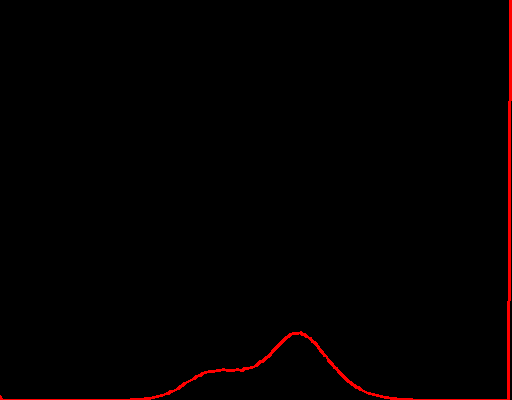
\includegraphics[width=\textwidth]{img2/hist_3_median_3_final_img2.png}
        \begin{center}
        	\textbf{Uniform surfaces}
        \end{center}
        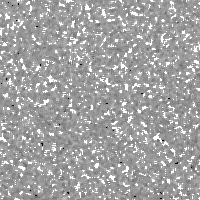
\includegraphics[width=\textwidth]{img2/rect_3_median_3_final_img2.png}\\[0.1cm]
        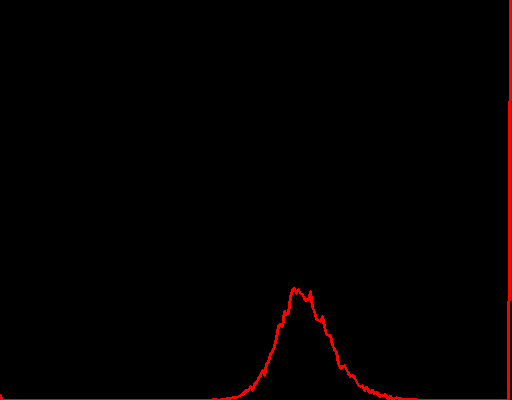
\includegraphics[width=\textwidth]{img2/hist_rect_3_median_3_final_img2.png}
        \caption{\lstinline|ksize = 3|}
        \label{fig:img2_kernel3}
    \end{subfigure}
    \begin{subfigure}[b]{0.24\textwidth}
        \includegraphics[width=\textwidth]{img2/median5.png}\\[0.1cm]
        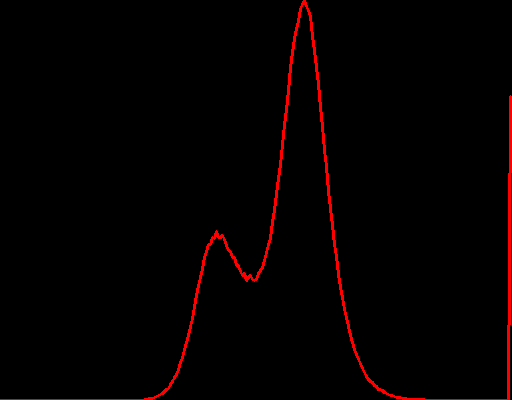
\includegraphics[width=\textwidth]{img2/hist_5_median_5_final_img2.png}
        \begin{center}
        	\text{ }
        \end{center}
        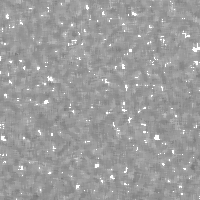
\includegraphics[width=\textwidth]{img2/rect_5_median_5_final_img2.png}\\[0.1cm]
        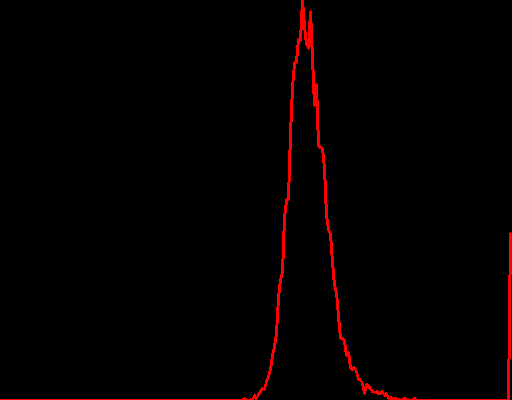
\includegraphics[width=\textwidth]{img2/hist_rect_5_median_5_final_img2.png}
        \caption{\lstinline|ksize = 5|}
        \label{fig:img2_kernel5}
    \end{subfigure}
    \begin{subfigure}[b]{0.24\textwidth}
        \includegraphics[width=\textwidth]{img2/median7.png}\\[0.1cm]
        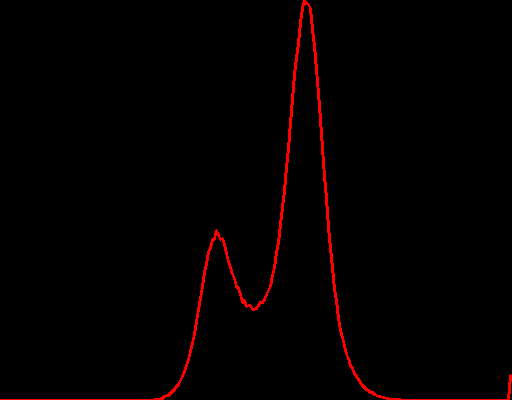
\includegraphics[width=\textwidth]{img2/hist_7_median_7_final_img2.png}
        \begin{center}
        	\text{ }
        \end{center}
        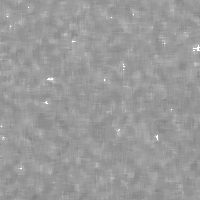
\includegraphics[width=\textwidth]{img2/rect_7_median_7_final_img2.png}\\[0.1cm]
        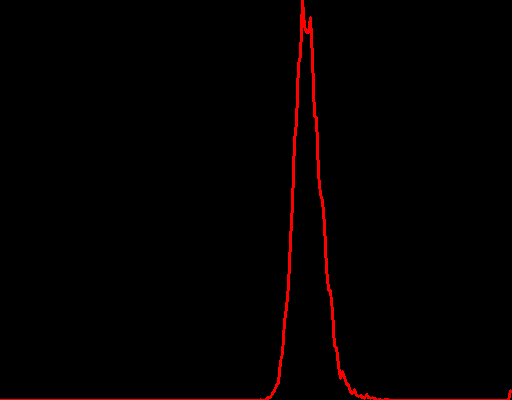
\includegraphics[width=\textwidth]{img2/hist_rect_7_median_7_final_img2.png}
        \caption{\lstinline|ksize = 7|}
        \label{fig:img2_kernel7}
    \end{subfigure}
    \begin{subfigure}[b]{0.24\textwidth}
        \includegraphics[width=\textwidth]{img2/median9.png}\\[0.1cm]
        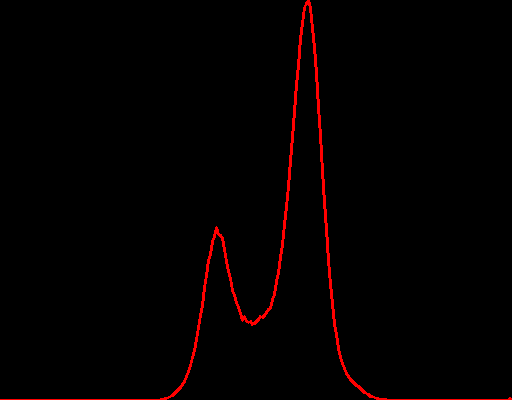
\includegraphics[width=\textwidth]{img2/hist_9_median_9_final_img2.png}
        \begin{center}
        	\text{ }
        \end{center}
        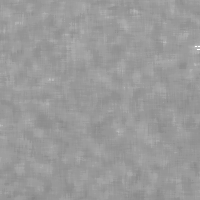
\includegraphics[width=\textwidth]{img2/rect_9_median_9_final_img2.png}\\[0.1cm]
        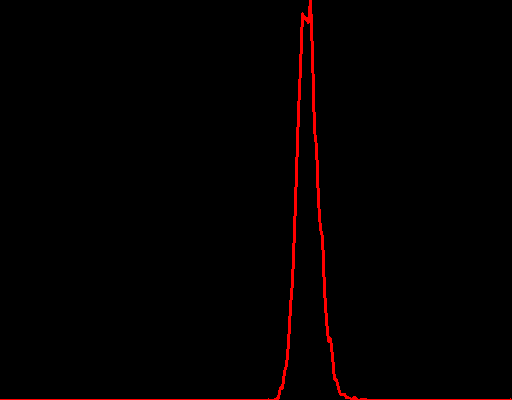
\includegraphics[width=\textwidth]{img2/hist_rect_9_median_9_final_img2.png}
        \caption{\lstinline|ksize = 9|}
        \label{fig:img2_kernel9}
    \end{subfigure}
    \caption{Analysis of image 2 -- Median filter}\label{fig:img2}
\end{figure}

\begin{figure}[H]
    \centering
    \begin{subfigure}[b]{0.28\textwidth}
        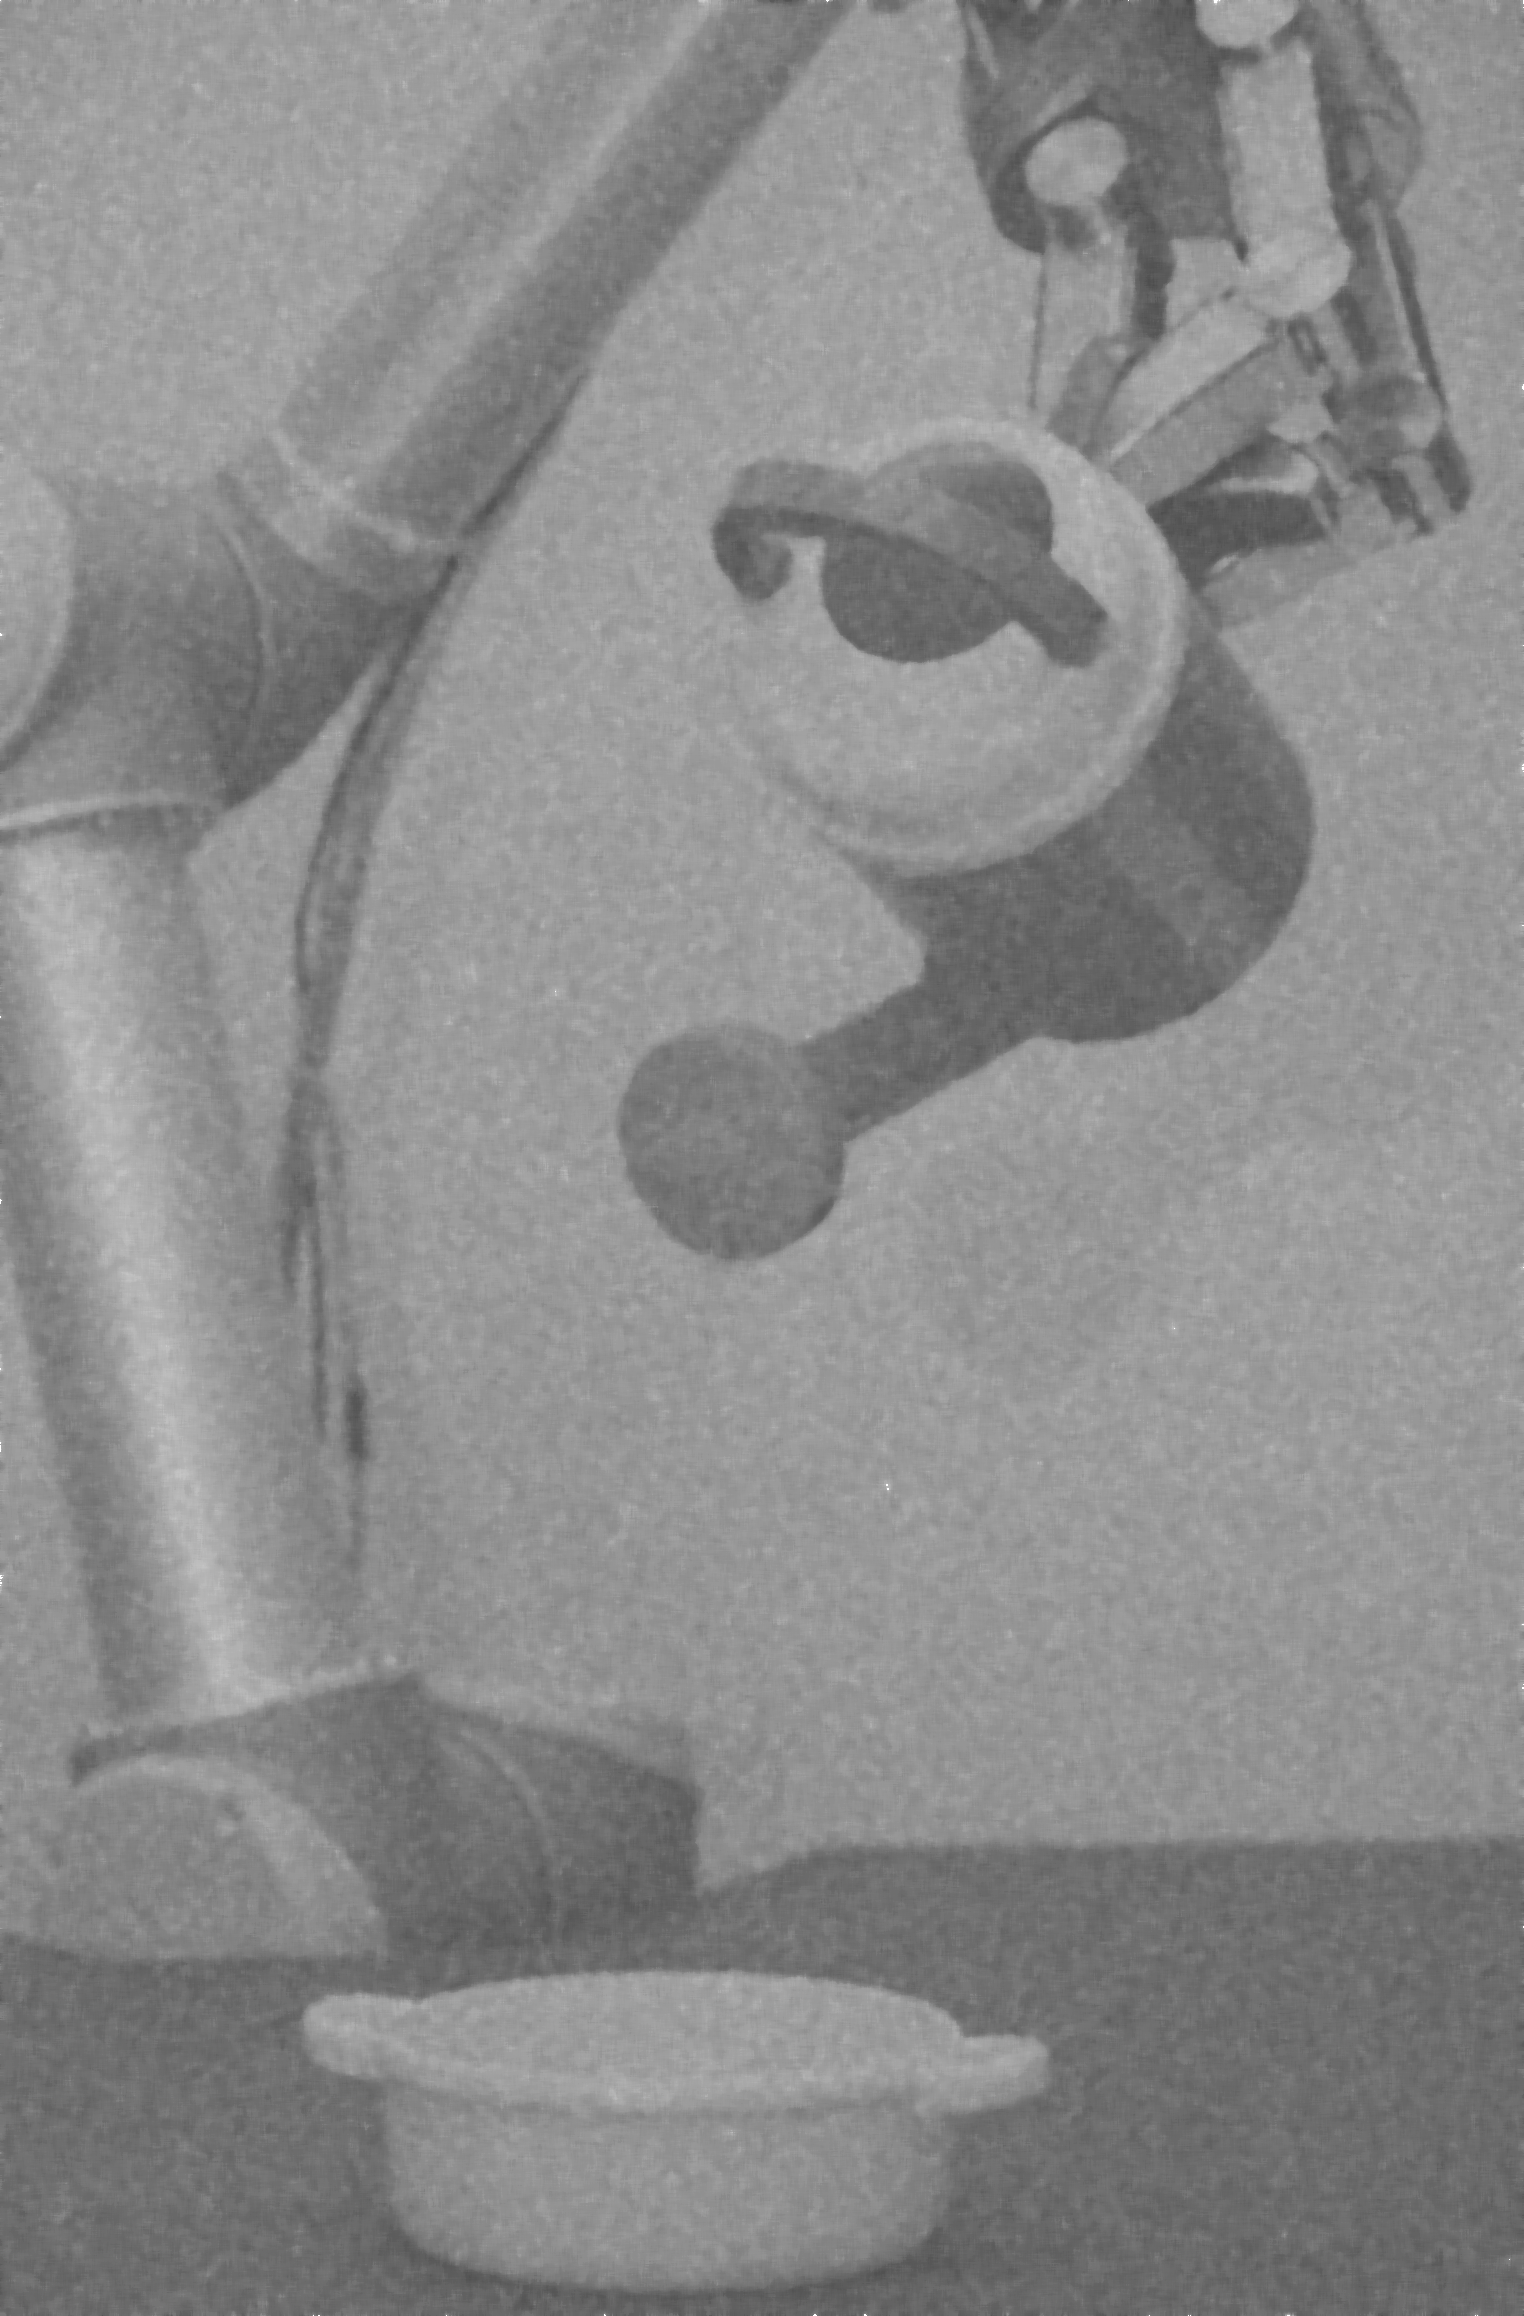
\includegraphics[width=\textwidth]{img2/median.png}\\[0.1cm]
        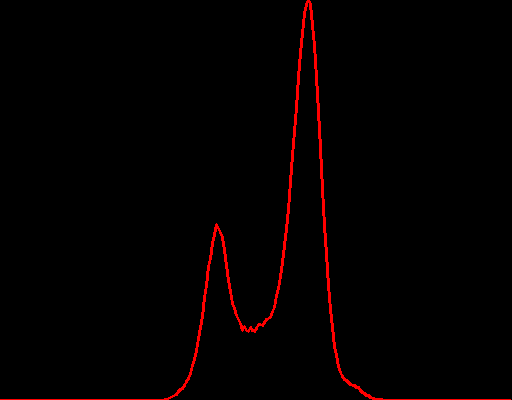
\includegraphics[width=\textwidth]{img2/hist_11_median_11_final_img2.png}
        \begin{center}
        	\textbf{Uniform surfaces}
        \end{center}
        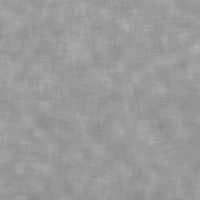
\includegraphics[width=\textwidth]{img2/rect_11_median_11_final_img2.png}\\[0.1cm]
        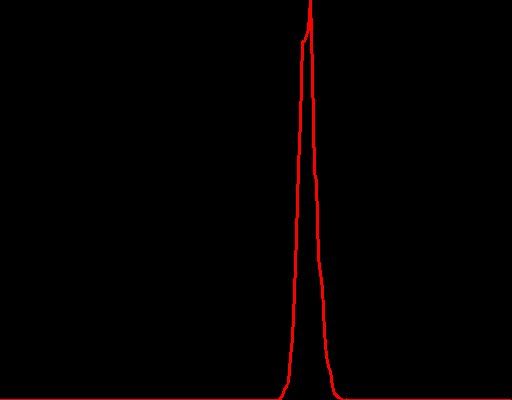
\includegraphics[width=\textwidth]{img2/hist_rect_11_median_11_final_img2.png}
        \caption{\lstinline|ksize = 11|}
        \label{fig:img2_kernel11}
    \end{subfigure}
    \begin{subfigure}[b]{0.28\textwidth}
        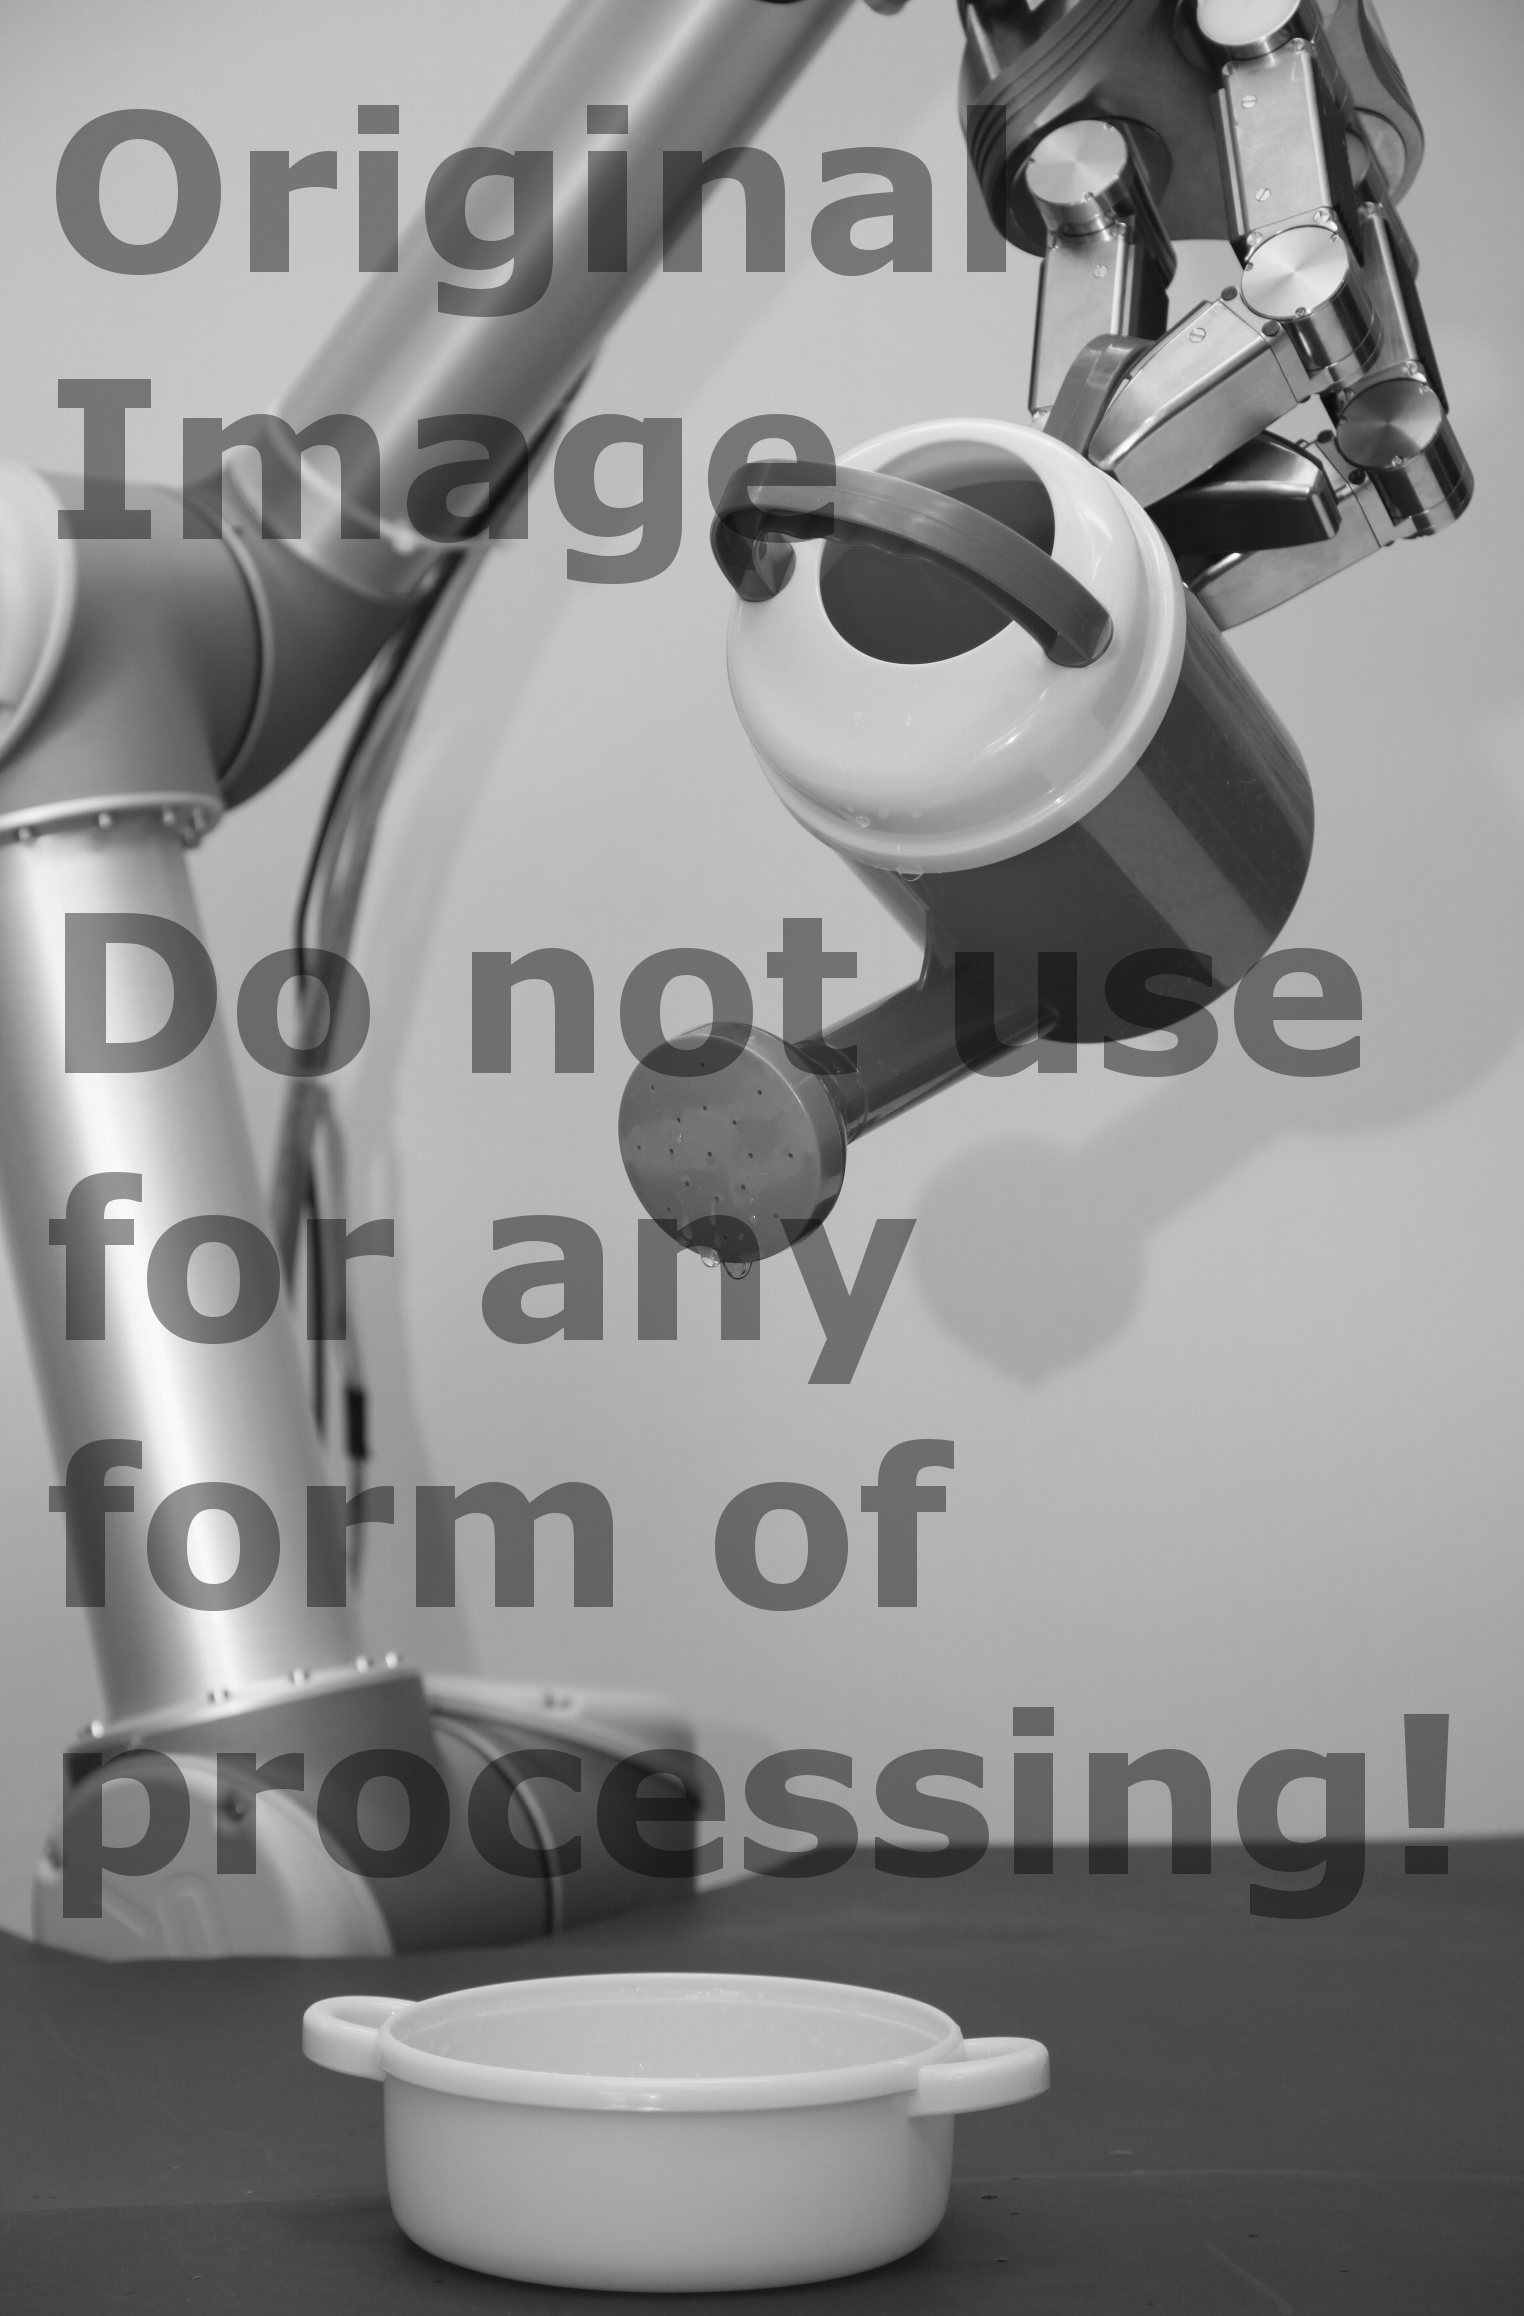
\includegraphics[width=\textwidth]{org.png}\\[0.1cm]
        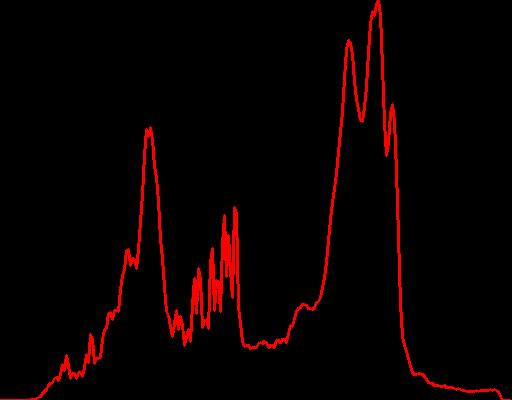
\includegraphics[width=\textwidth]{img2/hist_eee_org_res_total.png}
        \begin{center}
        	\text{ }
        \end{center}
        
\includegraphics[width=\textwidth]{img2/rect_eee_org_res_total.png}\\[0.1cm]
        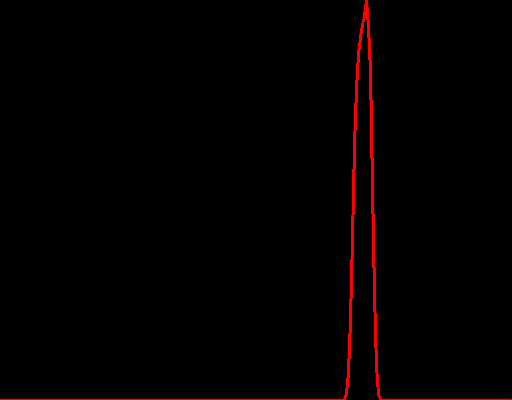
\includegraphics[width=\textwidth]{img2/hist_rect_eee_org_res_total.png}
        \caption{Original}
        \label{fig:img2_org}
    \end{subfigure}
    \begin{subfigure}[b]{0.28\textwidth}
        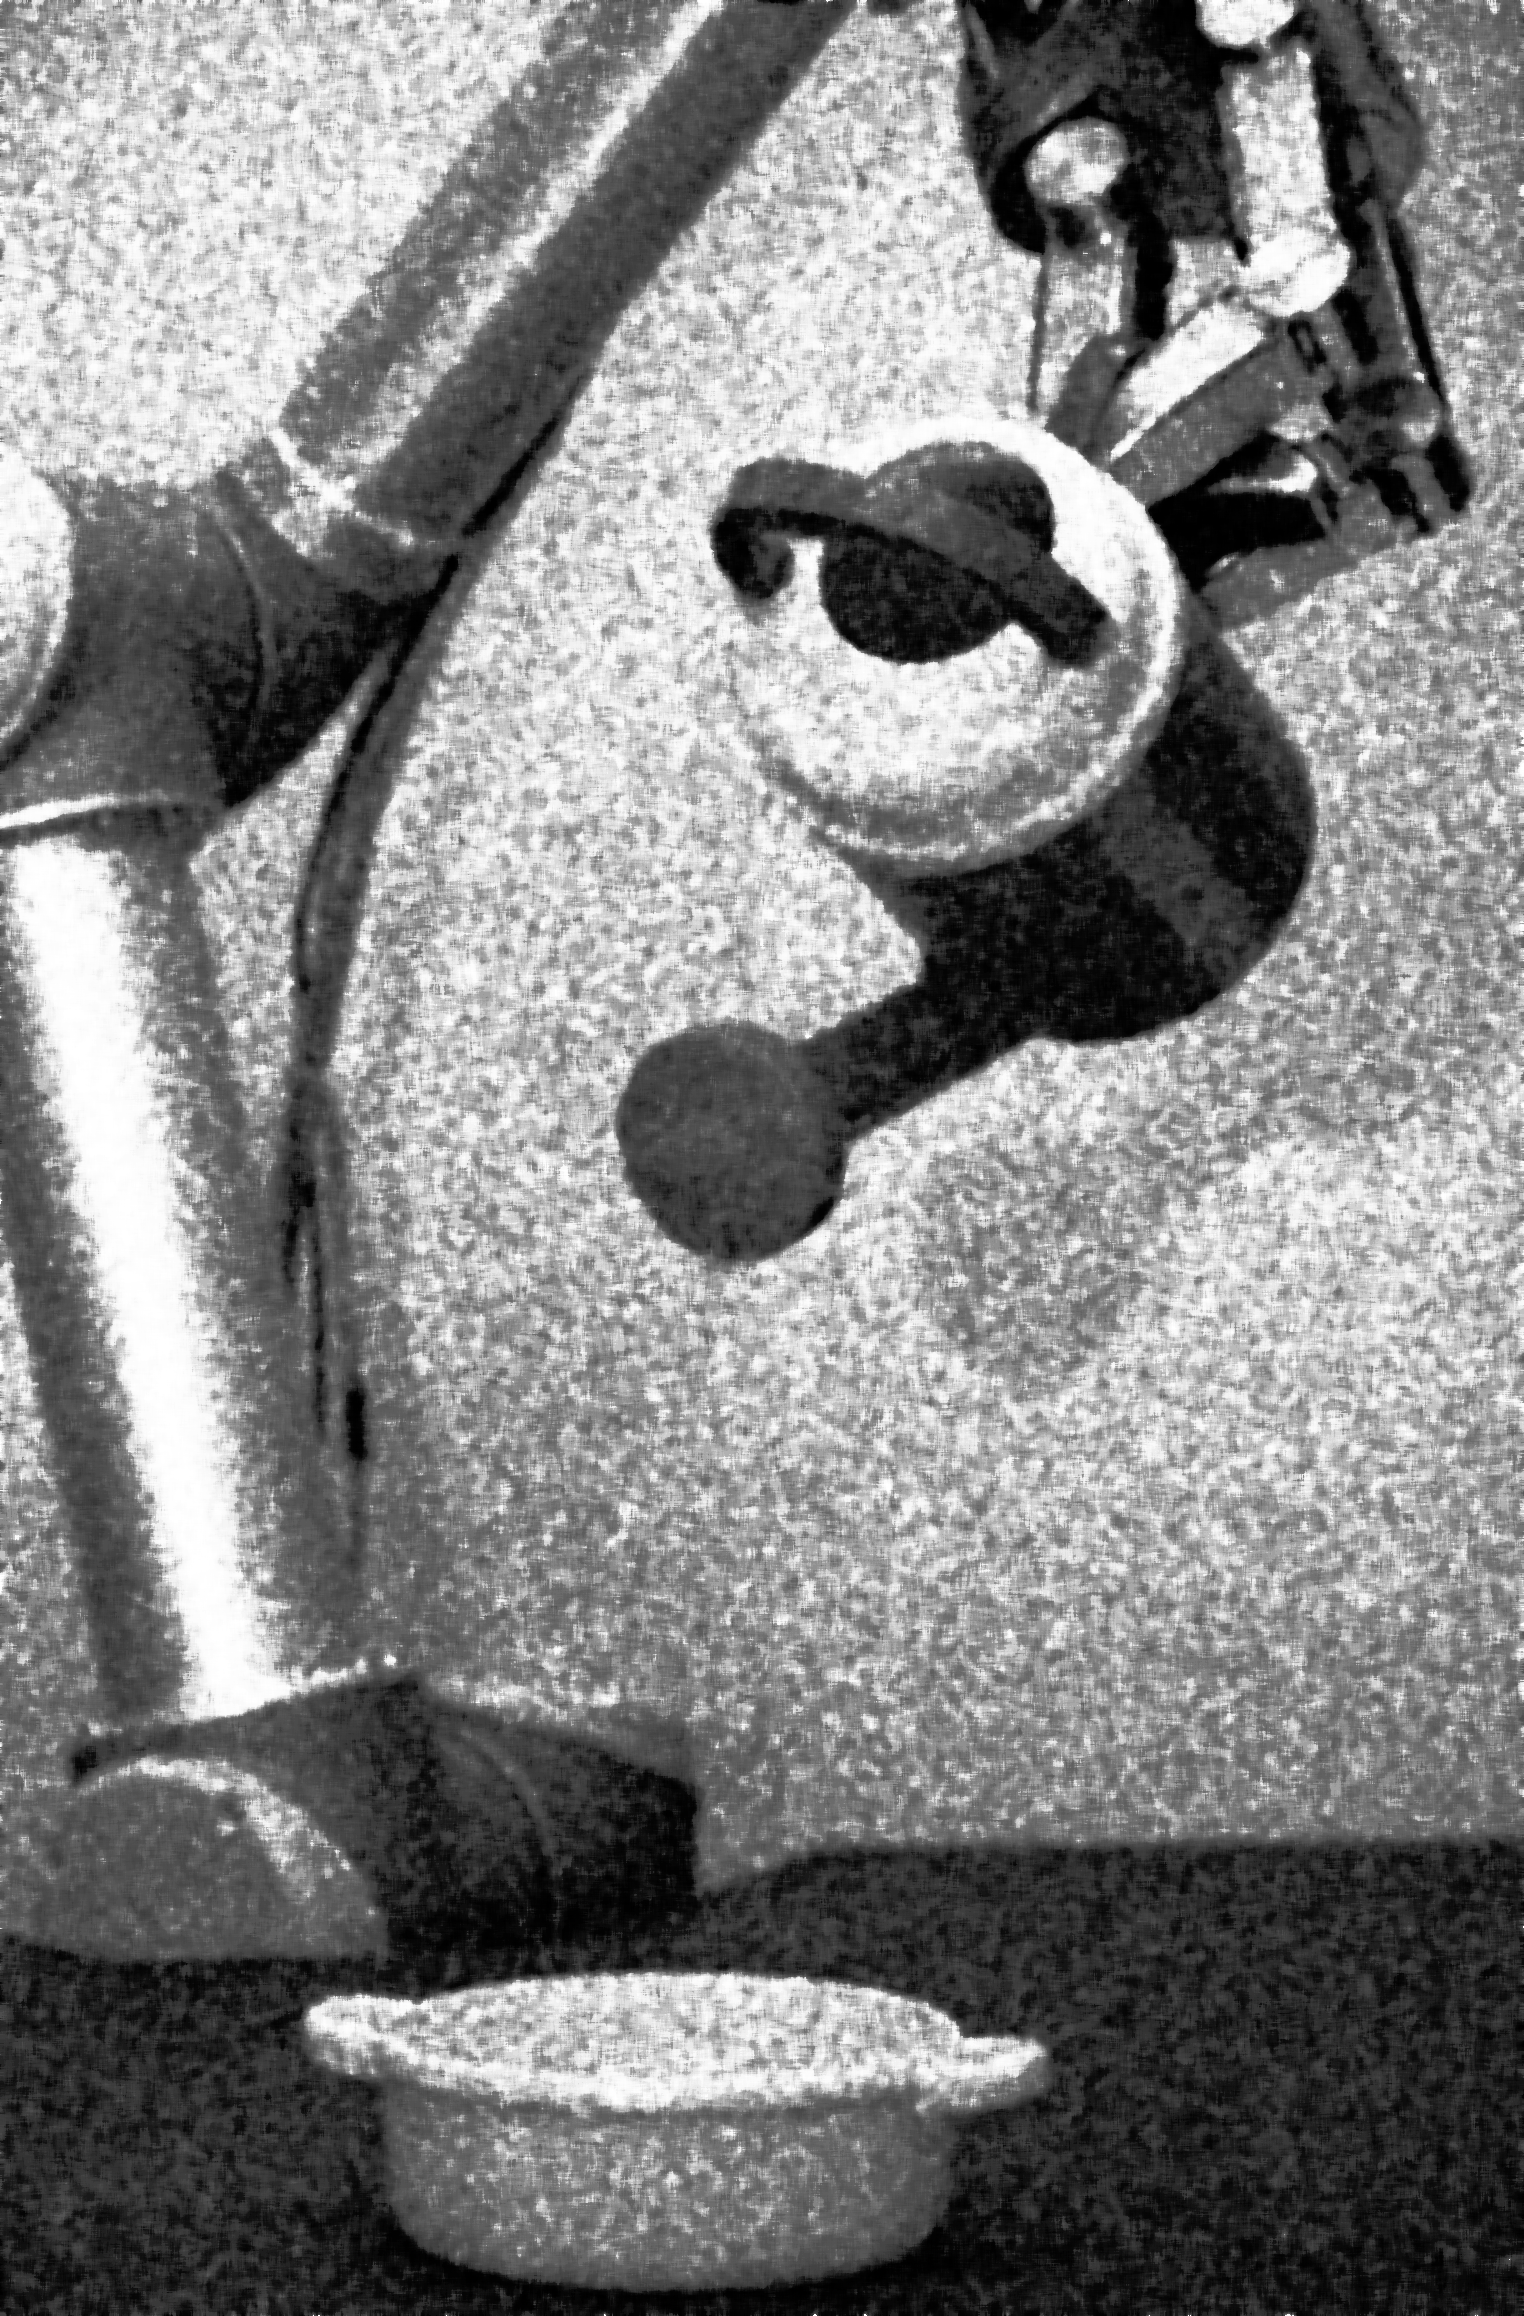
\includegraphics[width=\textwidth]{img2/eqlMedian.png}\\[0.1cm]
        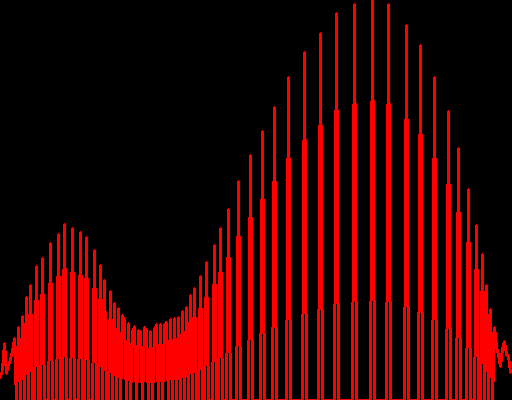
\includegraphics[width=\textwidth]{img2/hist_eee_eql_res_total.png}
        \begin{center}
        	\text{ }
        \end{center}
        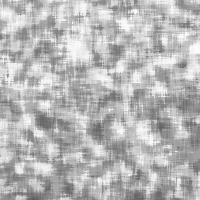
\includegraphics[width=\textwidth]{img2/rect_eee_eql_res_total.png}\\[0.1cm]
        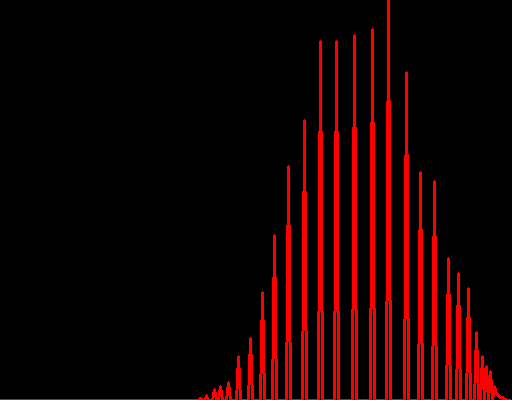
\includegraphics[width=\textwidth]{img2/hist_rect_eee_eql_res_total.png}
        \caption{Equalized}
        \label{fig:img2_histEq}
    \end{subfigure}
    \caption{Analysis of image 2}\label{fig:img2}
\end{figure}

\subsection{Adaptive Median Filter (AMF)}
An other approach for removing the salt--and--pepper noise from image \ref{fig:img2_add_test_e} is applying an AMF, which basically keeps the filter as small as possible during runtime in order to avoid extreme values. Figure \ref{fig:img2_add1} shows the image after the AMF is applied, and from its histogram can it be concluded that all the salt--and--pepper noise is removed, but the image is still filled with some kind of white noise, like Gaussian noise (figure \ref{fig:noise_gaussian}) or uniform noise (figure \ref{fig:noise_uniform}). I order to determine this, an uniform surface is analysed, and by comparing the its histogram with the noise types on figure \ref{fig:noise_examples_img3}, it looks like the white noise is Gaussian noise. I order to reduce this noise, the OpenCV function below is used:
\begin{center}
	\lstinline|void GaussianBlur(InputArray src, OutputArray dst, Size ksize, double sigmaX, double sigmaY=0, int borderType=BORDER_DEFAULT)|\footnote{\url{http://docs.opencv.org/2.4/modules/imgproc/doc/filtering.html\#gaussianblur}}
\end{center}
Figure \ref{fig:img2_add2}, \ref{fig:img2_add3} and \ref{fig:img2_add4} shows three different \lstinline|ksize| of the kernel, and an \lstinline|ksize=5| is considered the best fit for removing the Gaussian noise, without blurring the image more than necessary is. 

\begin{figure}[H]
    \centering
    \begin{subfigure}[b]{0.22\textwidth}
        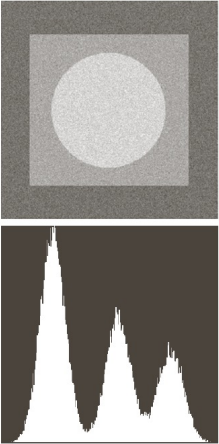
\includegraphics[width=\textwidth]{img3/noise_g.png}
        \caption{Gaussian noise}
        \label{fig:noise_gaussian}
    \end{subfigure}
    \begin{subfigure}[b]{0.2175\textwidth}
        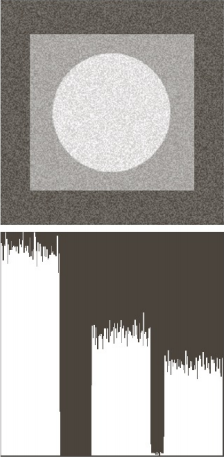
\includegraphics[width=\textwidth]{img3/noise_u.png}
        \caption{Uniform noise}
        \label{fig:noise_uniform}
    \end{subfigure}
    \caption{Examples of different noise models}
    \label{fig:noise_examples_img3}
\end{figure}

Comparing the result of using either the median filter (figure \ref{fig:img2_kernel11}) or the adaptive (figure \ref{fig:img2_add3}), the results are almost similar, but the approaches are different. A high kernel size is need for the median filter, but the same is not the case for the adaptive median filter, so the result is the same, but the computation time will differ.  

\begin{figure}[H]
    \centering
    \begin{subfigure}[b]{0.24\textwidth}
        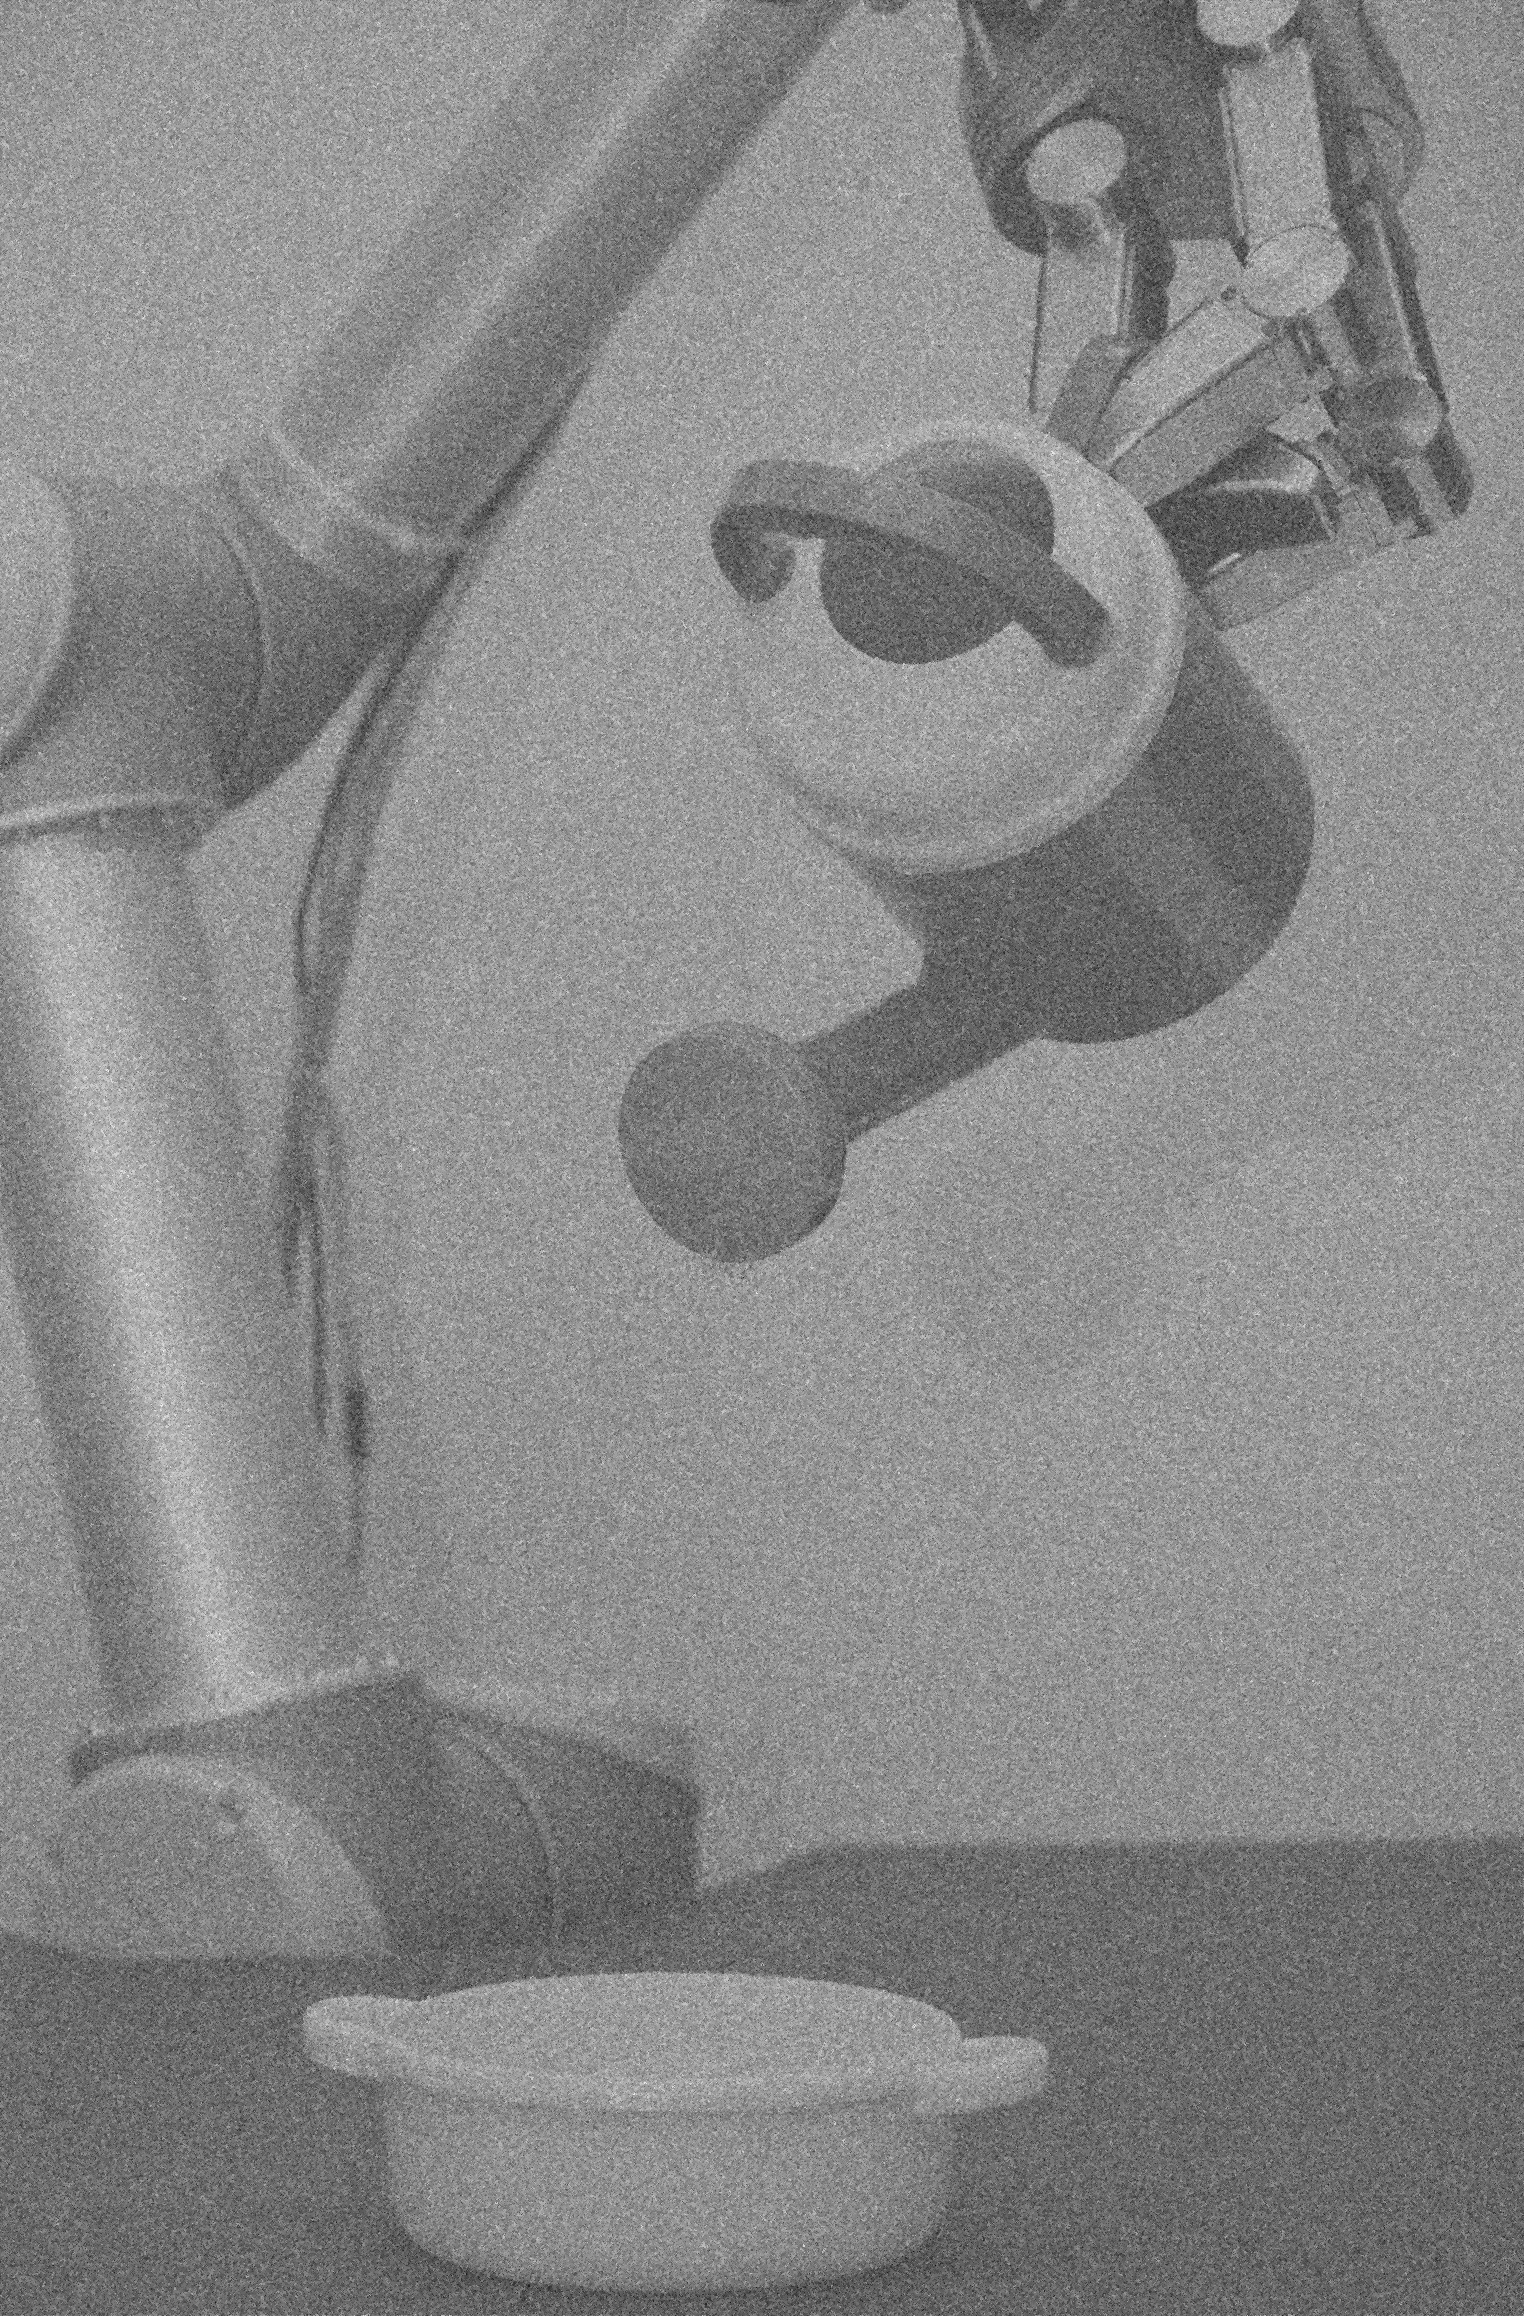
\includegraphics[width=\textwidth]{img2/adaptive_3_final_img2.png}\\[0.1cm]
        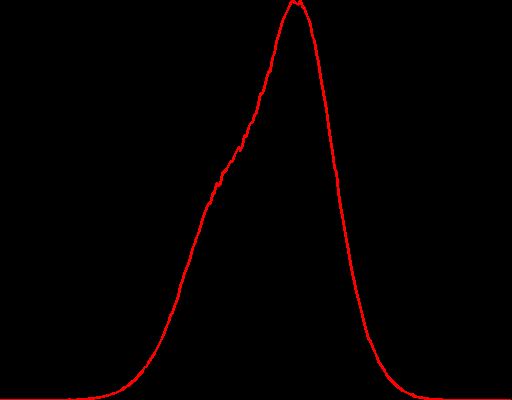
\includegraphics[width=\textwidth]{img2/hist_1_adaptive_test_2_final_img2.png}
        \begin{center}
        	\textbf{Uniform surfaces}
        \end{center}
        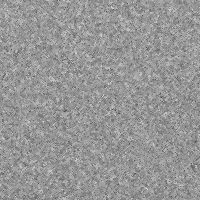
\includegraphics[width=\textwidth]{img2/rect_1_adaptive_test_2_final_img2.png}\\[0.1cm]
        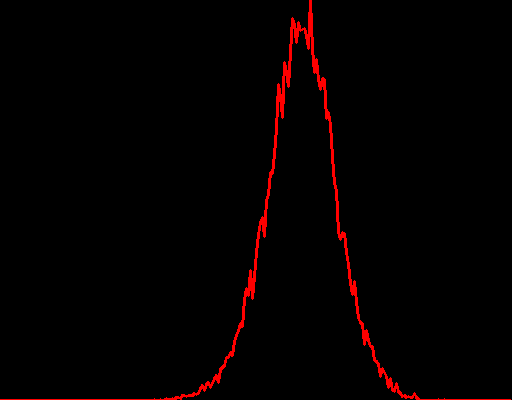
\includegraphics[width=\textwidth]{img2/hist_rect_1_adaptive_test_2_final_img2.png}
        \caption{Image 2 w/AMF}
        \label{fig:img2_add1}
    \end{subfigure}
    \begin{subfigure}[b]{0.24\textwidth}
        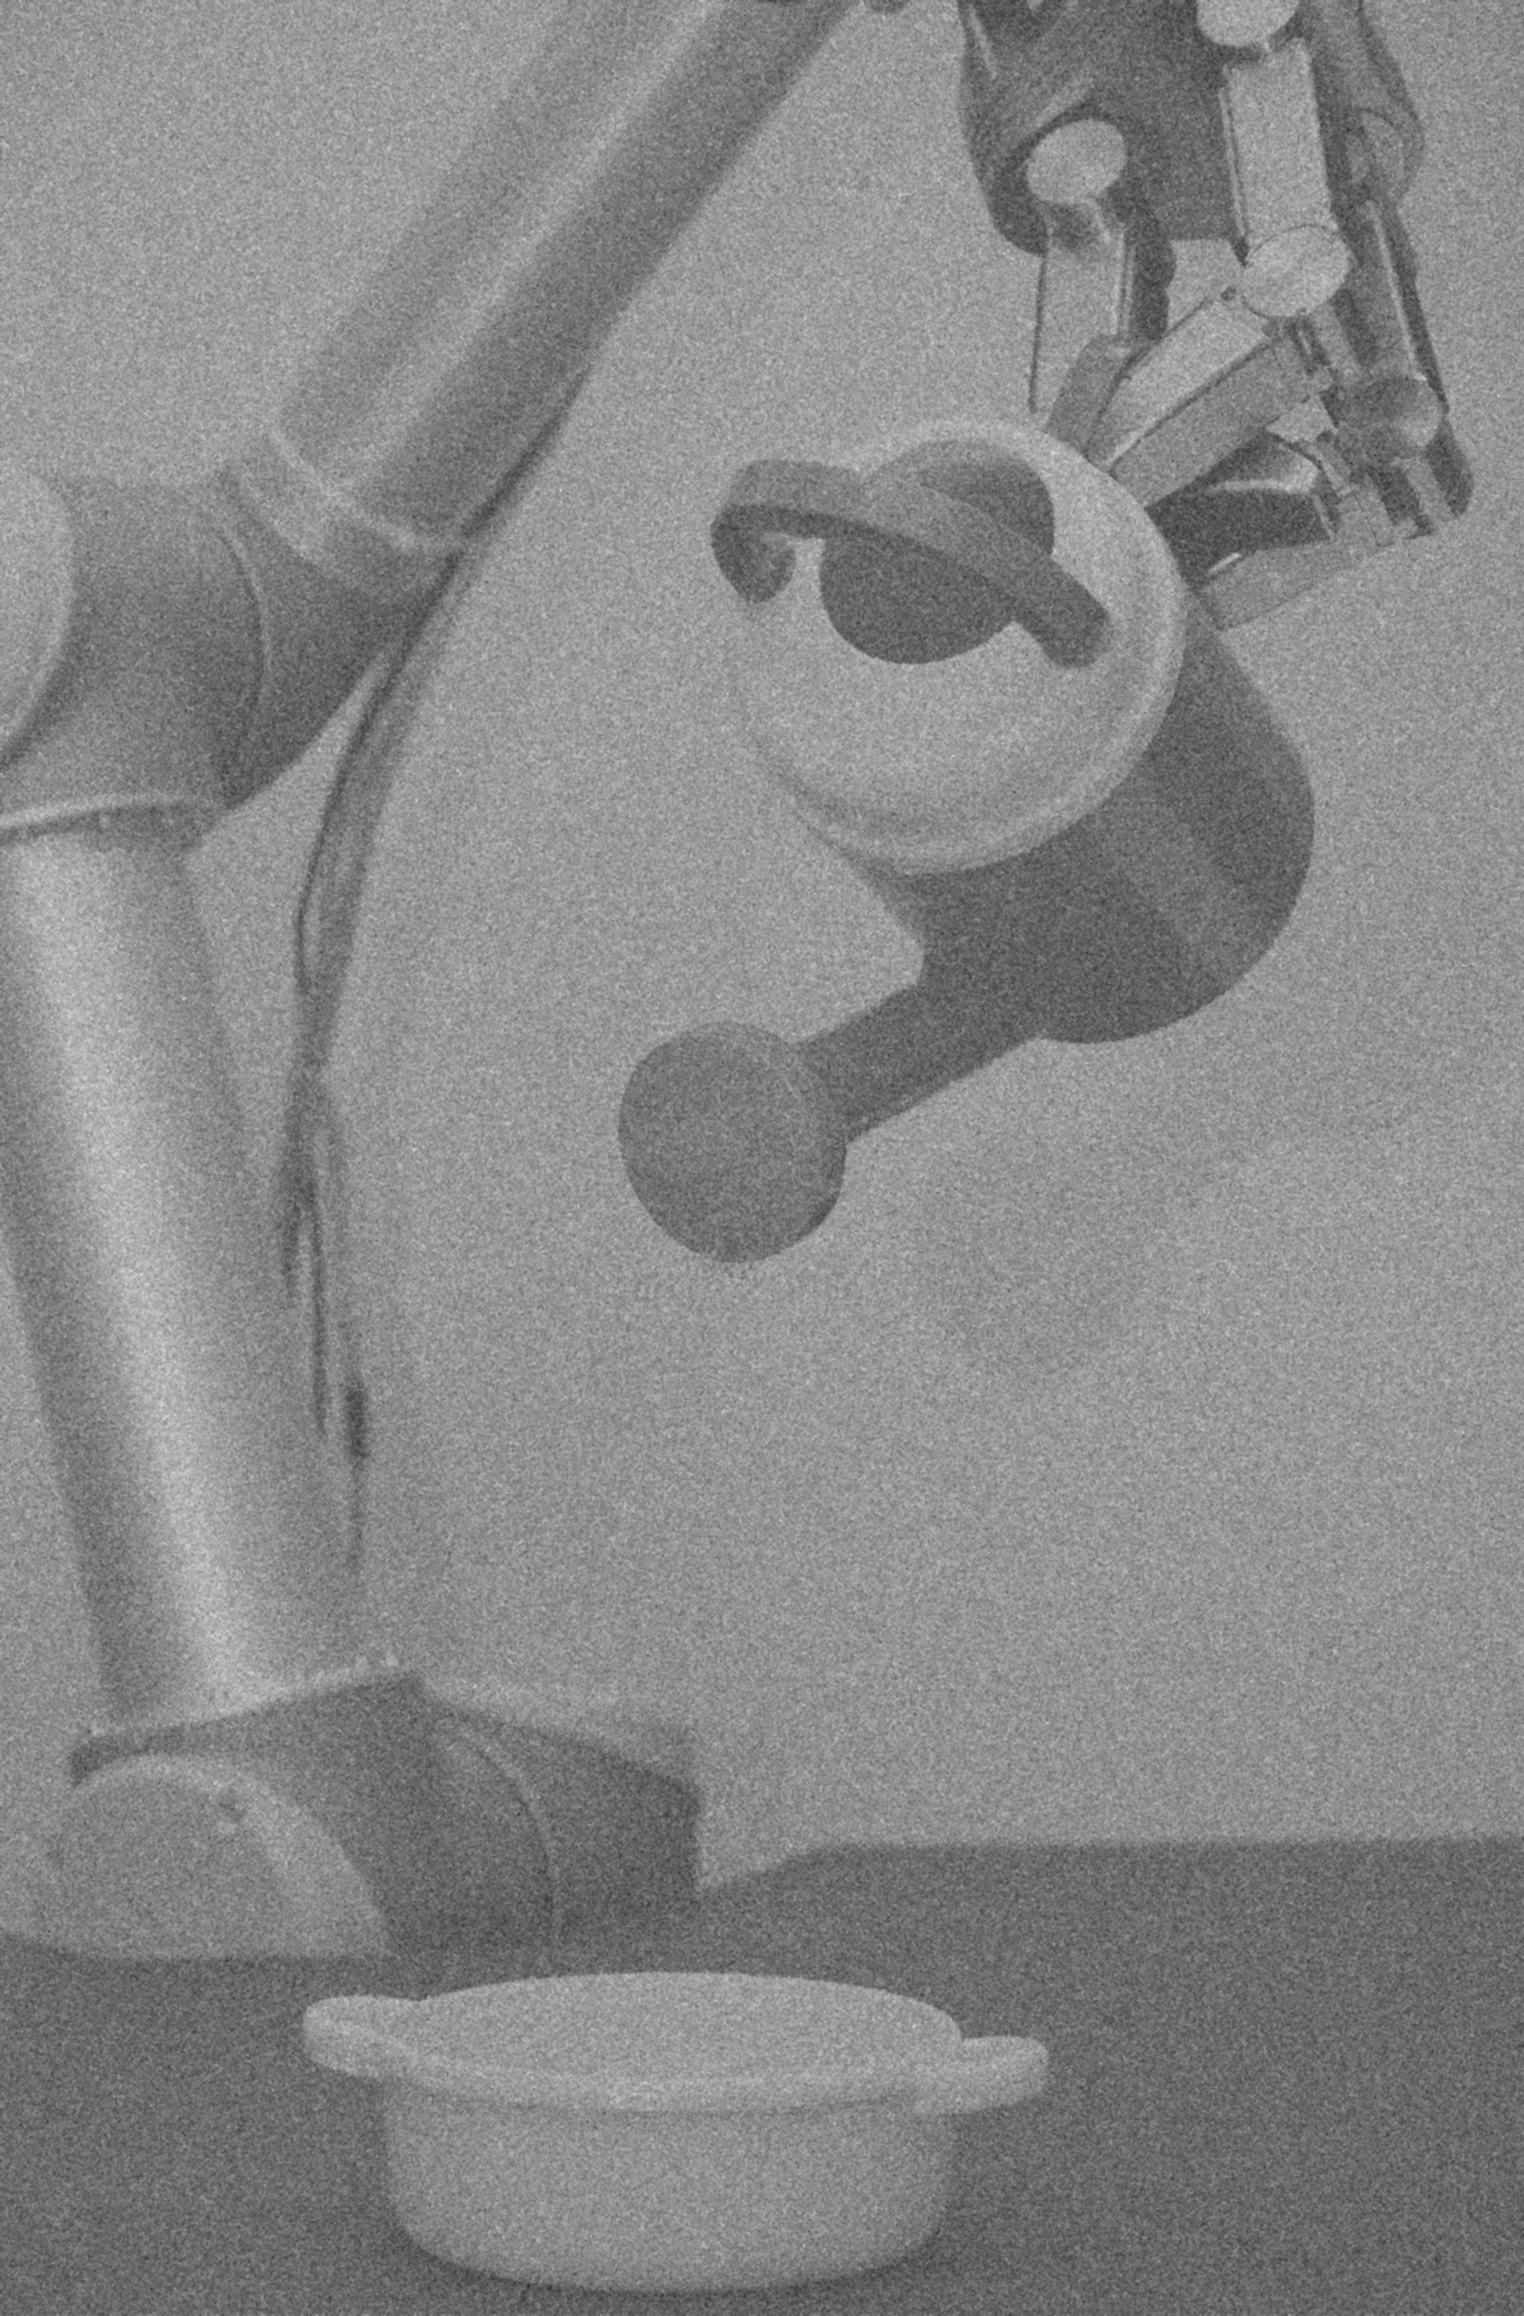
\includegraphics[width=\textwidth]{img2/adaptive_3_test_final_img2.png}\\[0.1cm]
        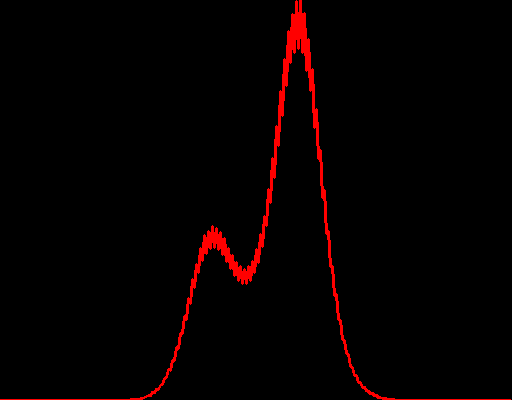
\includegraphics[width=\textwidth]{img2/hist_2_adaptive_3_test_final_img2.png}
        \begin{center}
        	\textbf{ }
        \end{center}
        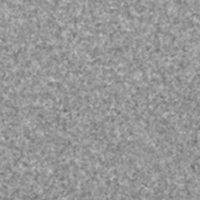
\includegraphics[width=\textwidth]{img2/rect_2_adaptive_3_test_final_img2.png}\\[0.1cm]
        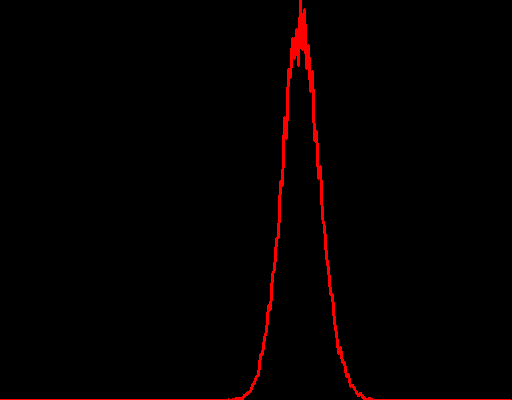
\includegraphics[width=\textwidth]{img2/hist_rect_2_adaptive_3_test_final_img2.png}
        \caption{\lstinline|ksize = 3|}
        \label{fig:img2_add2}
    \end{subfigure}
    \begin{subfigure}[b]{0.24\textwidth}
        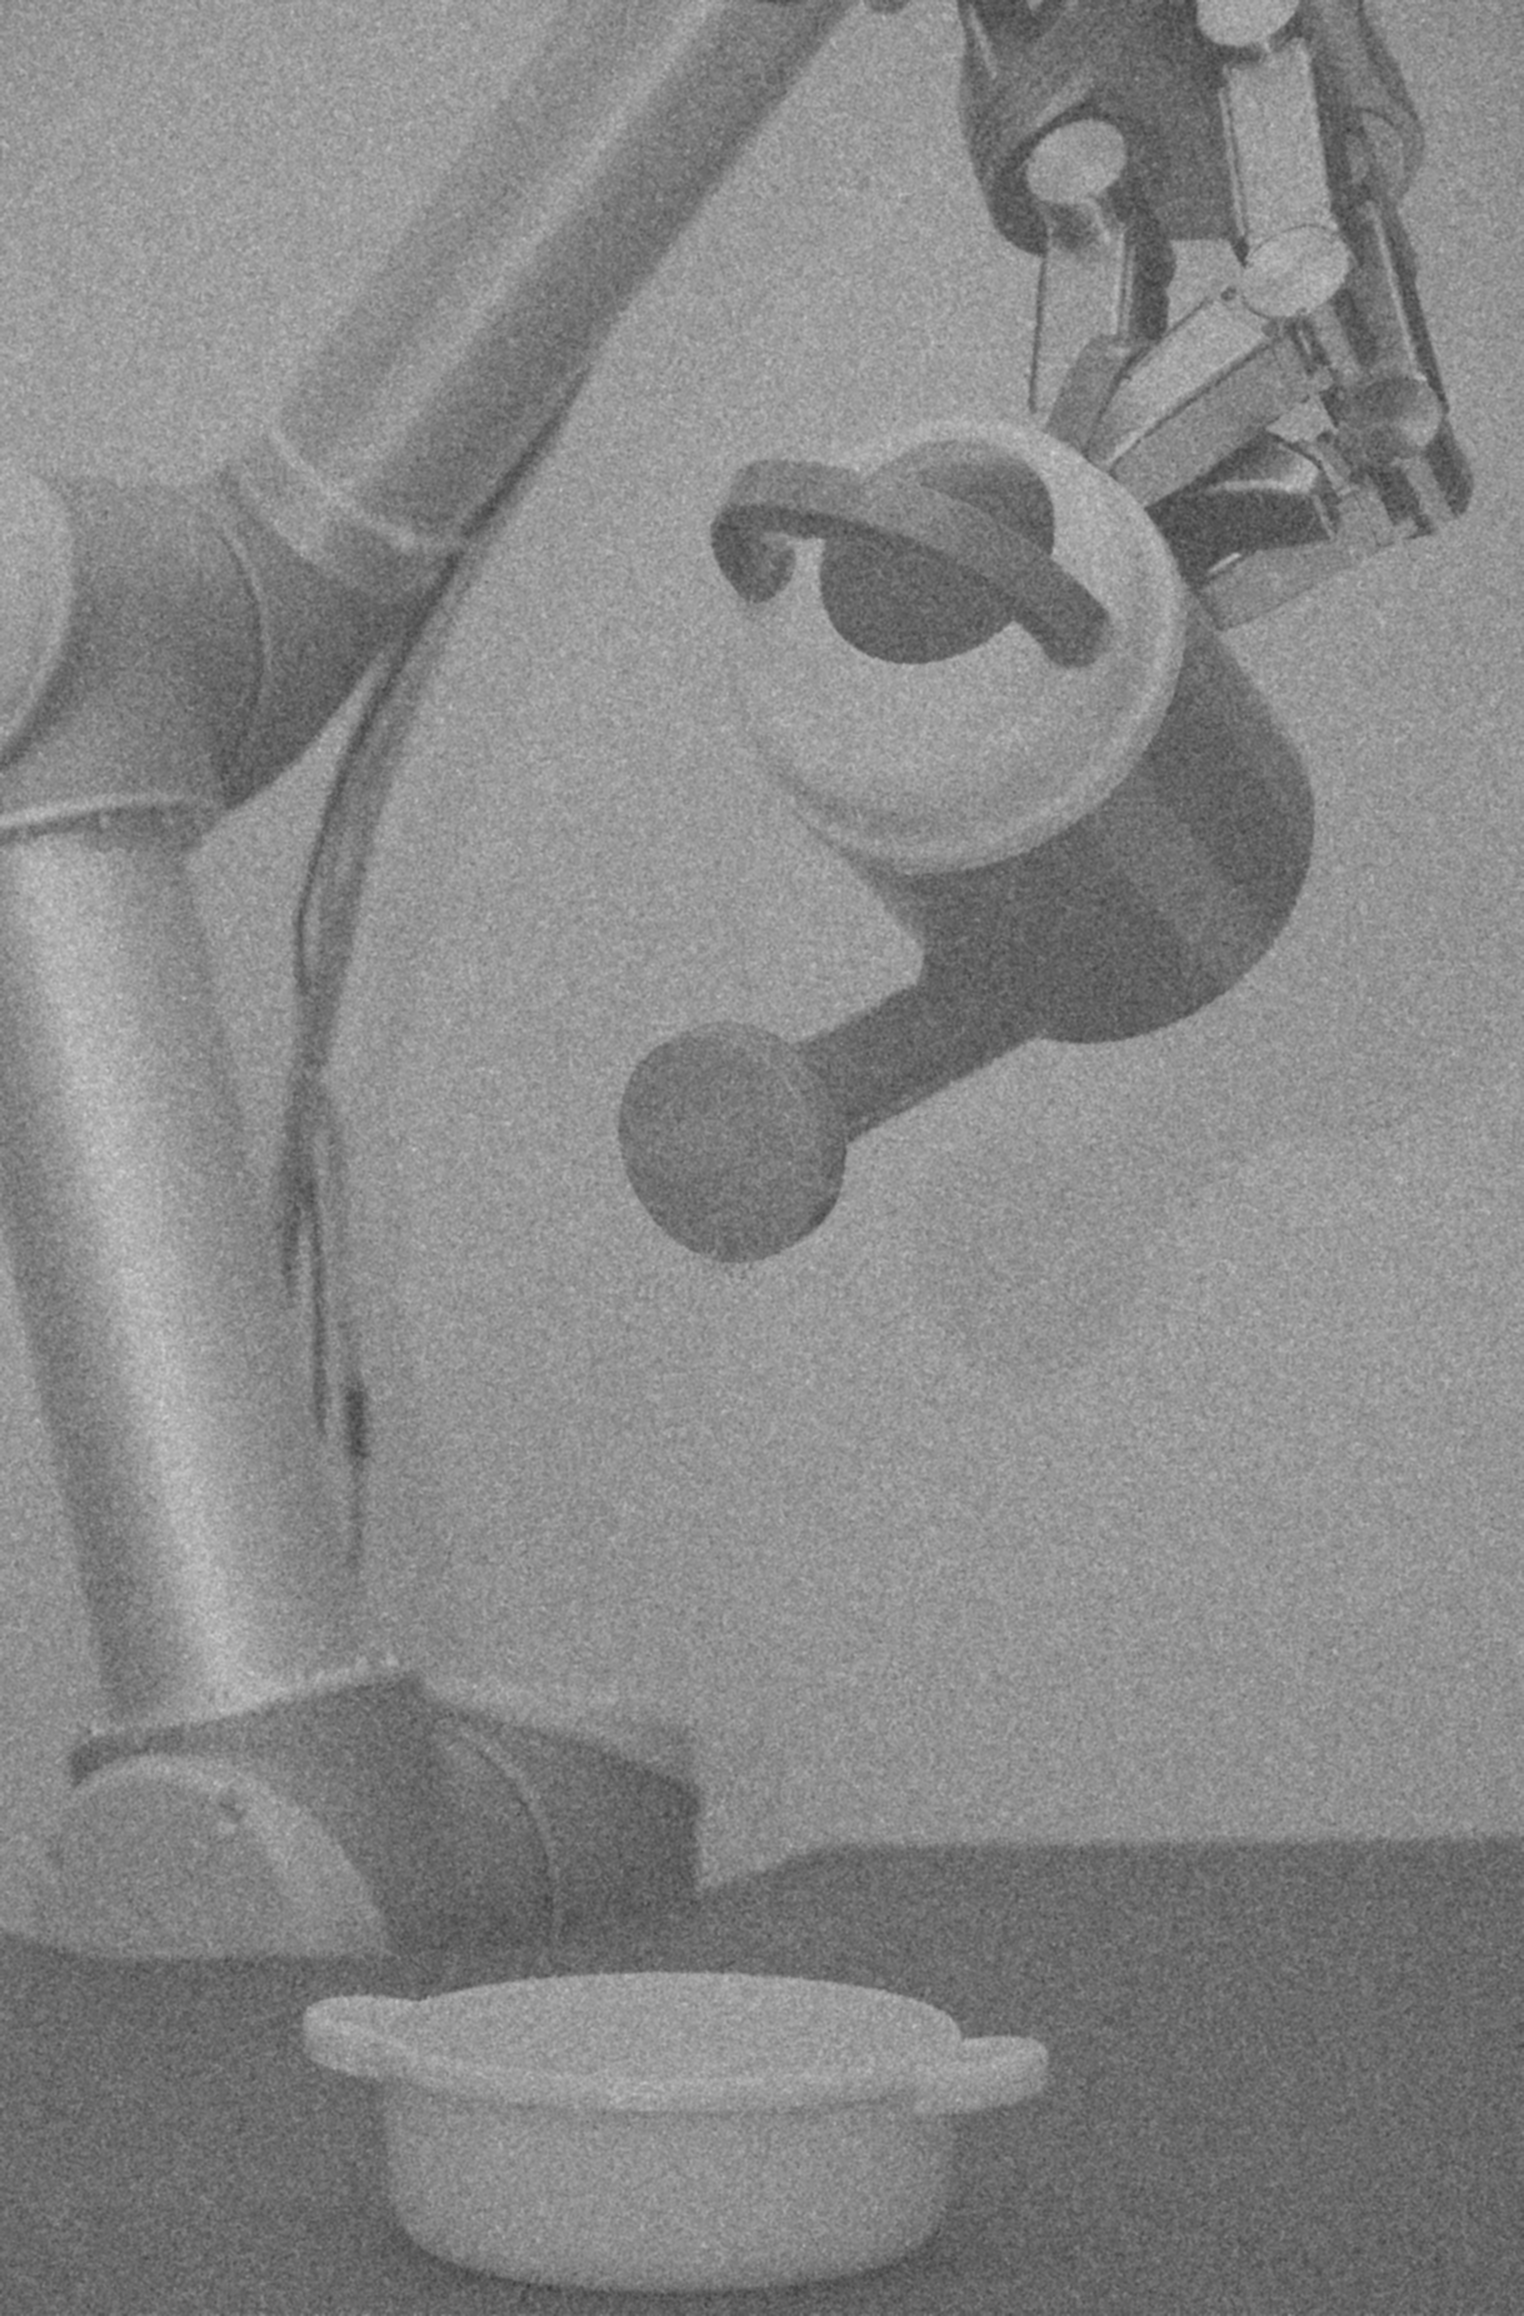
\includegraphics[width=\textwidth]{img2/adaptive_5_test_final_img2.png}\\[0.1cm]
        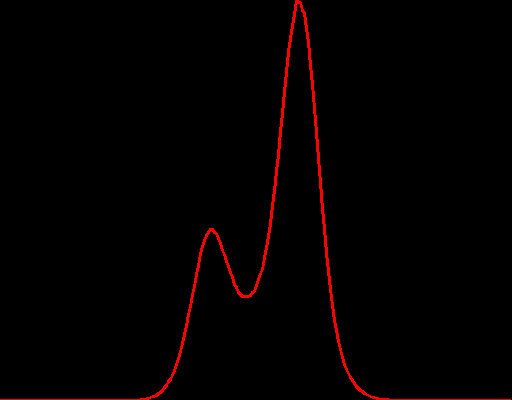
\includegraphics[width=\textwidth]{img2/hist_2_adaptive_5_test_final_img2.png}
        \begin{center}
        	\textbf{ }
        \end{center}
        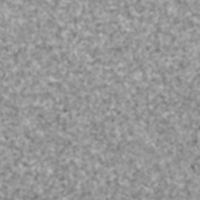
\includegraphics[width=\textwidth]{img2/rect_2_adaptive_5_test_final_img2.png}\\[0.1cm]
        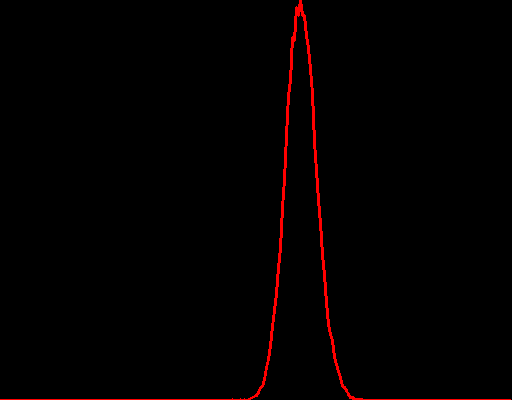
\includegraphics[width=\textwidth]{img2/hist_rect_2_adaptive_5_test_final_img2.png}
        \caption{\lstinline|ksize = 5|}
        \label{fig:img2_add3}
    \end{subfigure}
    \begin{subfigure}[b]{0.24\textwidth}
        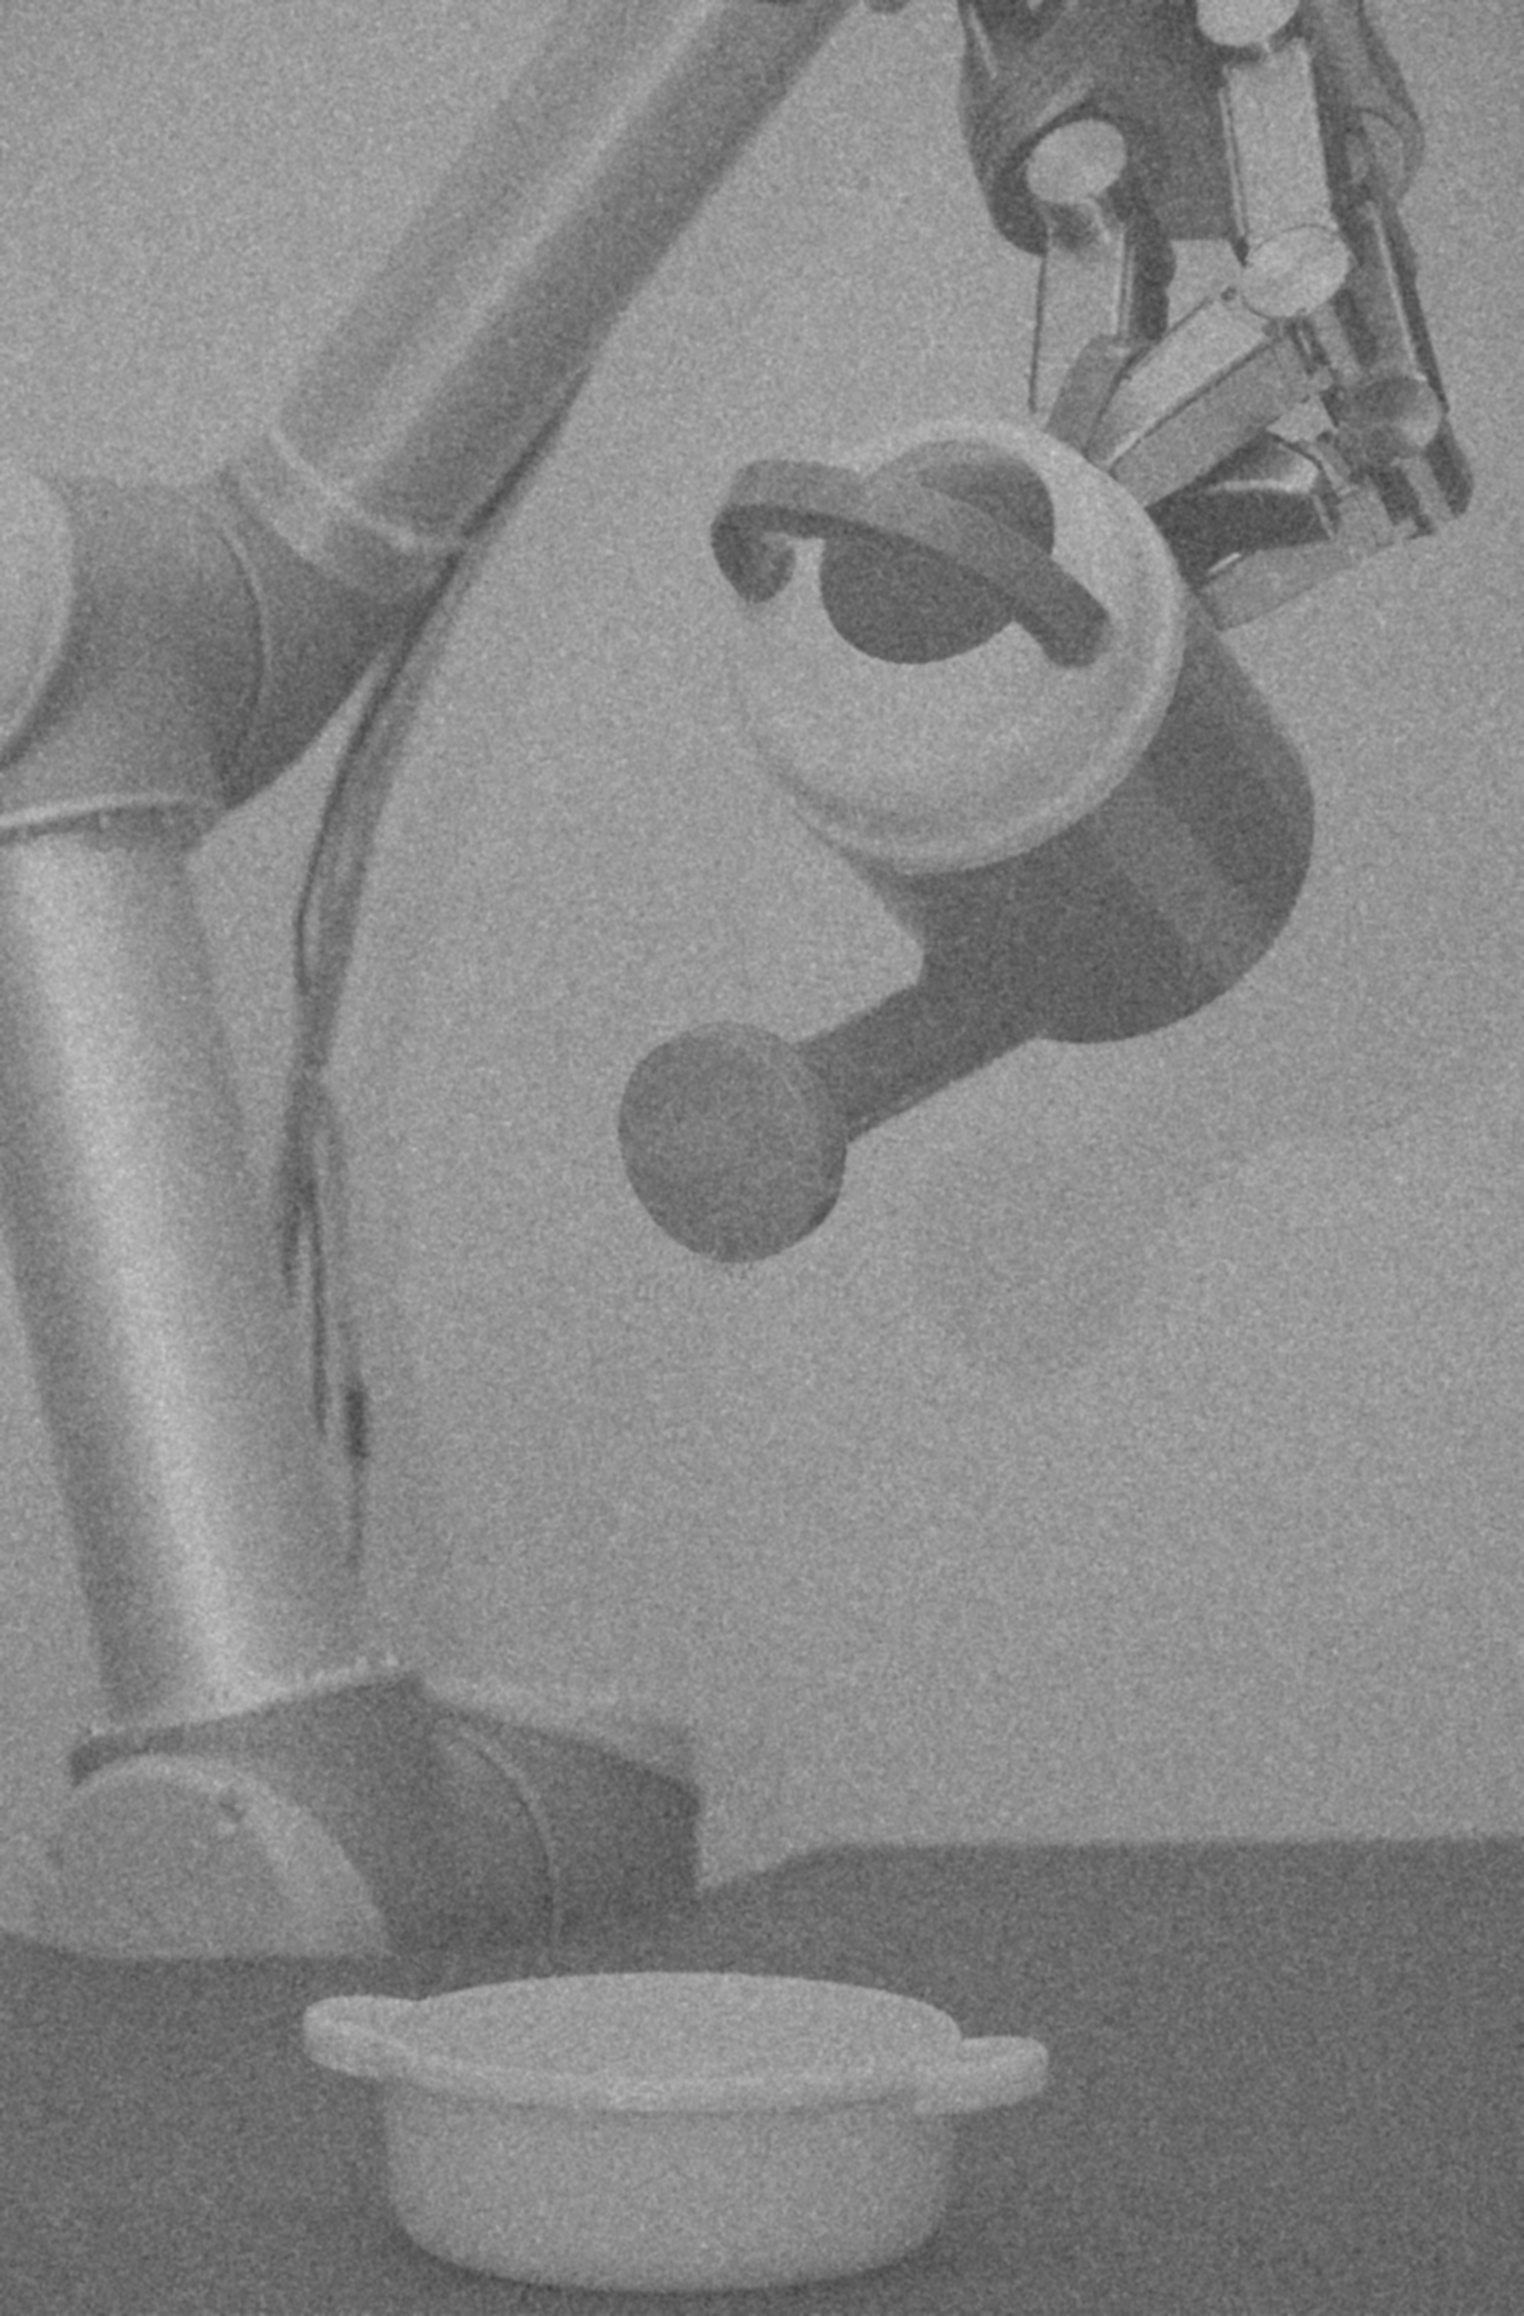
\includegraphics[width=\textwidth]{img2/adaptive_7_test_final_img2.png}\\[0.1cm]
        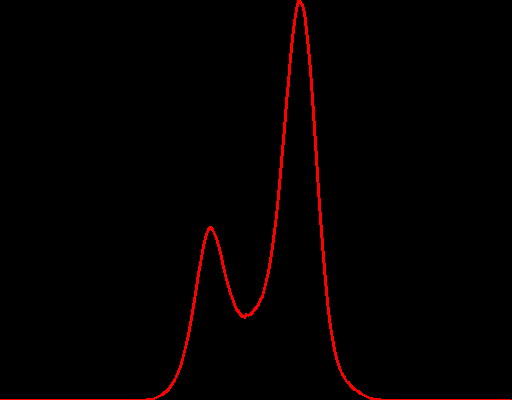
\includegraphics[width=\textwidth]{img2/hist_2_adaptive_7_test_final_img2.png}
        \begin{center}
        	\textbf{ }
        \end{center}
        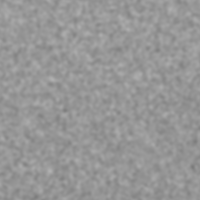
\includegraphics[width=\textwidth]{img2/rect_2_adaptive_7_test_final_img2.png}\\[0.1cm]
        \includegraphics[width=\textwidth]{img2/hist_rect_2_adaptive_7_test_final_img2.png}
        \caption{\lstinline|ksize = 7|}
        \label{fig:img2_add4}
    \end{subfigure}
    \caption{Analysis of image 2 -- Adaptive Median filter and Gaussian Blur}\label{fig:img2_add_test_e}
\end{figure}

